% ****** Start of file aapmsamp.tex ******
%
%   This file is part of the AAPM files in the AAPM distribution for REVTeX 4-2.
%   Version 4.2a of REVTeX, January 2015
%
%   Copyright (c) 2015 American Association of Physicists in Medicine (AAPM).
%
%   See the AAPM README file for restrictions and more information.
%
%   Three character codes for review purposes:


\documentclass[%
 portrait,
 aapm,
 mph,%
 amsmath,amssymb,
%preprint,%
 reprint,%
%author-year,%
%author-numerical,%
]{revtex4-2}

\usepackage{graphicx}% Include figure files
\usepackage{dcolumn}% Align table columns on decimal point
\usepackage{bm}% bold math
\usepackage{wrapfig}%This package allows for image wrapping
%\usepackage{incgraph,tikz}%Let's me make an image take a full page
\usepackage{pdfpages}%Okay, maybe this will work. Update: Breaks the document RE-update: All good with the follwing lines. 
\makeatletter
\AtBeginDocument{\let\LS@rot\@undefined}
\makeatother


%This package enables Kanji characters to be recognized in our bibtex file. 
%It throws a fit otherwise
\usepackage{CJKutf8}


%\usepackage[mathlines]{lineno}% Enable numbering of text and display math
%\modulolinenumbers[5]% Line numbers with a gap of 5 lines
%\linenumbers\relax % Commence numbering lines



\usepackage{hyperref}%Allows for hyperlinks. The stuff below sets some defaults.
\hypersetup{
    colorlinks=true,
    linkcolor=blue,
    filecolor=magenta,      
    urlcolor=cyan,
    citecolor=red
}
 
\urlstyle{same}

\begin{document}

\preprint{AAPM/123-QED}

\title[Team 25 PDR]
{L'SPACE Team 25 \\ Preliminary Design Review\footnote{Error!}}% Force line breaks with \\
%\thanks{Footnote to title of article.}

\author{
\includegraphics[width=100pt]{Logos/nasaLogo.png}
\includegraphics[width=100pt]{Logos/lucyLogo.jpg}
\includegraphics[width=90pt]{Logos/lspaceLogo.jpg}}
\affiliation{} 

\author{Israel De Los Santos}%
 \affiliation{ 
Southwestern Oklahoma State University, Manufacturing Engineering Technology
}%
 
\author{Miryah Adair}%
 \affiliation{ 
Southwestern Oklahoma State University, Engineering Technology
}%

\author{Jacob Miller}
 \affiliation{%
Southwestern Oklahoma State University, Computer Science
}%

\author{Travis Pilati}%
 \affiliation{ 
Oklahoma State University, Aerospace/Mechanical Engineering
}%

\author{Bridgette Davey}%
 \affiliation{ 
Monmouth College, Physics
}%


\author{Declan A. Crego}%
 \affiliation{ 
Monmouth College, Physics/Pre-engineering
}%

\author{Charles Sleeper}%
 \affiliation{ 
Southwestern Oklahoma State University, Computer Science
}%

\author{Johnson Seri}%
 \affiliation{ 
Tulsa Community College/Oklahoma State University, Mechanical Engineering/Physics
}%

\date{\today}% It is always \today, today,
             %  but any date may be explicitly specified

\begin{abstract}
\textbf{Abstract:} \\
This Preliminary Design Review (PDR) details a proposed unmanned mission to Mars with the purpose of finding water ice to be used in feed-stock for future manned missions. This mission will be relatively inexpensive and light so that it may accompany an already planned mission, but the data gleaned will still be extremely valuable. The mission will make use of an Alpha Proton X‐Ray Spectrometer (APXS) and a mini ground penetrating radar to assess the presence and usability of water ice at the selected location. The payload will be delivered to the surface via a custom descent and landing system and will be held by a custom lander.
\newpage
%
\end{abstract}

%\keywords{Suggested keywords}%Use showkeys class option if keyword
                              %display desired
\maketitle



%Begin section I
\section{\label{sec:level1}Summary of PDR Report:%\protect\\ The line
%break was forced \lowercase{via} \textbackslash\textbackslash%
}

%Begin section 1.1
\subsection{Team Summary}
The organizational structure of the team is centralized. The Project Manager oversees the two Deputy Project Managers, who each coordinate the engineering team and science team. The science team is responsible for developing the scientific experiment, and research goals for the mission, while the engineering team is responsible for developing the means to do just that. 

%1.1.1
\subsubsection{College and University Names}
\begin{itemize}
    \item Oklahoma State University (OSU)
    \item Southwestern Oklahoma State University (SWOSU)
    \item Monmouth College
    \item Tulsa Community College / OSU
\end{itemize}

%1.1.2
\subsubsection{Locations}
\textbf{Oklahoma State University:} Stillwater, Oklahoma \\ 
\textbf{SWOSU:} Weatherford, Oklahoma\\ 
\textbf{Monmouth College: }Monmouth, Illinois \\ 
\textbf{Tulsa Community College:} Tulsa, Oklahoma \\ 
%1.1.3
\subsubsection{List of relevant expertise on team}
\begin{Large}\textbf{Project Manager}\end{Large}\\ \\
Israel De Los Santos:
\begin{itemize}
    \item Leaderhip Skills
    \item Time Management Skills
    \item Motivational Speaker
    \item Mediator
    \item Executive Decision Maker
\end{itemize}

\begin{Large}\textbf{Engineering Team}\end{Large}\\ \\
Travis Pilati:
\begin{itemize}
    \item Keeping people on task
    \item Landing and descent systems design
    \item Computer Assisted Design
    \item Mock landing simulations
    \item Aerodynamic engineering skills
    \item General engineering questions consultant
    \item Science Team/Engineering coordination
\end{itemize}
Johnson Seri:
\begin{itemize}
    \item Drafting and design of Probe
    \item Computer Assisted Design
    \item Scientific instrument integration
    \item Instrument deployment mechanism
\end{itemize}
Miryah Adair:
\begin{itemize}
    \item Engineering Team Coordinator
    \item Drafting and design of probe
    \item Computer Assisted Design
    \item Scientific instrument integration
    \item Instrument deployment mechanism
\end{itemize}


\begin{Large}\textbf{Science Team}\end{Large}\\ \\
Jacob Miller:
\begin{itemize}
    \item Science Team Coordinator
    \item Task delegator
    \item Gantt chart coordinator
    \item \LaTeX
    \item Landing Site Selection
    \item Budgeting 
    \item Task integration
    \item JMARS
    \item Finization of PDR
\end{itemize}
Declan Crego:
\begin{itemize}
    \item Scientific Instrument Selection
    \item Public outreach
    \item Landing site selection
    \item Document writing
\end{itemize}
Charles Sleeper:
\begin{itemize}
    \item Data organization
    \item Hierarchy creation
    \item Document writing
    \item Landing site selection
\end{itemize}
Bridgette Davey:
\begin{itemize}
    \item Telecommunicator
    \item Scientific probe selection and experiment design
    \item JMARS and landing site selection
    \item Attendance accountability
    \item Visual Systems Design and Scientific Instrument Integration
    \item Documentation
    \item Budgeting
    \item Public outreach
\end{itemize}


%1.2
\subsection{Descent Summary}
As the limitations for this mission make conventional descent and landing systems non-viable, older National Aeronautics and Space Administration (NASA) missions served as the inspiration for this system. 
%1.2.1
\subsubsection{Description of entry, descent, and landing sequence}
The lander will approach the Martian atmosphere at approx 6 km/s.  Upon entering the atmosphere the Lander's heat shield will absorb a large amount of the energy and slow down to a few hundred meters per second.  At that point the parachute will deploy and slow the lander down to a few tens of meters per second.  Small rockets attached to the lander will then fire to slow the craft to a standstill a about 10-20 meters off the ground.  The parachute will detach and fly off by the thrust of the small rockets.  After a specified amount of time the landing craft will inflate its airbags that will allow for a semi-soft landing.  The crafts outer shell will then open to allow the lander to conduct its mission \cite{raiszadeh2011mars}. 
%1.3
\subsection{Lander and Payload Summary}
Upon landing and becoming stationary, the airbags will begin an equalization period, deflating over the course of about 90 minutes. After this time, the lander can begin deploying. Due to its pyramidal shape, it will always deploy with the instruments in the correct configuration. After deployment, the instruments are free to begin their work.
%1.3.1
\subsubsection{Description of each mission element}
The alpha particle x-ray spectrometer (APXS) is an instrument our probe will inherit from previous mars exploration rovers: Spirit, Opportunity, and Sojourner. The APXS instrument’s function will be to relay information about the chemical composition of glacial regolith mixture at our Probe’s landing sites. There are two main types of radiation APXS will use, alpha particles and x-ray waves \cite{APXS_NASA_Mars}. This instrument's head is only a mere 52 mm wide and 88 mm long. The overall weight is only .6 kg, and the power draw .4 W \cite{bruckner2003refined}. 

The mini ground penetrating radar (MGPR) is a relatively recent instrument developed by NASA's own Jet Propulsion Laboratory (JPL). It's primary function is to gather information about the subsurface of Mars. The instrument consists of 2 boards 5 cm wide, 10 cm long, and 2 cm tall. It weighs a total of .045 kg and draws 1 W of power \cite{kim2006miniature}. 
Although small and light, the mini ground penetrating radar provides excellent data. It has two configurations, one provides data from deeper levels (up to 50 m in depth) at moderate resolution, and the second which allows for shallow penetration (up to 5 m) at a finer resolution \cite{kim2012miniature}. 

%1.3.2
\subsubsection{Description of surface experiment deployment system}
As stated in the summary section, with the design of the lander there is little chance the lander will be in an incorrect configuration after deployment. It's pyramidal shape will cause it to righten itself even if it lands on it's side or back. Once this is completed, the scientific payload can begin deploying it's instruments. 

From here, mechanisms on the payload will deploy the instrument. The MGPR's antenna will extend from the rover, and the APXS will be attached to an arm that can be lowered onto the surface.

%1.3.3
\subsubsection{Summarize experiment and how science obtained furthers overall mission objectives}
The science experiment conducted by the instruments of the lander will begin by using the on-board Mini Ground Penetrating Radar. This instrument will give information about the immediate subsurface of Mars, including the quantity of ice in the immediate vicinity. Secondly, the APXS will be used to take several samples of the near-surface ice in the region. This instrument will give information about the quality of ice; if it is potable, water or \begin{math} CO_2 \end{math}, and other qualities. 

%Begin Section II
\section{\label{sec:level2}Evolution of Project}

%2.1
\subsection{Highlight All Changes Made Since the Initial Concept Was Identified and the Reason for those Changes}

%2.1.1
\subsubsection{Changes made to Descent and Lander Criteria}
The descent and lander criteria was fairly straightforward from the start. It needed to get the payload from orbit to the surface safely, a daunting task. As it was decided that landing safely was probably the most important aspect of the mission, the other aspects of the mission waited to get their exact criteria until the descent and lander system was being finalized. Initially, conventional landing methods were considered, but were quickly decided against. The fuel required was simply too heavy. So, the system currently detailed in section IV was devised. As it was clear the total weight was going to come out to about 2 kg, the criteria for the other sections were decided. 

%2.1.2
\subsubsection{Changes made to Payload Criteria}
Many options were initially considered for the payload. As the team deliberated, it was decided that it was important to be able to drill, and to analyze the chemical components of a sample. The drill was eventually ruled out, as all options were far too heavy. The team did select a Palm portable mass spectrometer as an instrument initially. However, as it became clear the landing system would take 2 kg, that tool was also ruled out to be too heavy. The payload was relegated to 3 kgs in total, 1.5 for instruments, and 1.5 for the rover. Once these were set, the current configurations were selected. Overall, budget was never an issue. 

%2.1.3
\subsubsection{Changes made to Mission Experiment Implementation Plan}
The experiment underwent several revisions as well, right along with the payload. The initial concept was a drill that would unearth subsurface ice, and a mass spec that would analyze that ice. A hot water drill seemed promising, but had to be removed due to weight restrictions, so the aforementioned experiment could not be performed. Without the drill, the team moved to just using a mass spec, combined with some sort of scraper that could remove dust. A mass spec could then analyze samples that way. However, this was once again, too heavy. Limited to less than 1.5 kg, the team developed the current experiment. 


%Begin Section III
\section{\label{sec:level3}Science Value}

%3.1
\subsection{Highlight the Science Payload and Value to Mission Objectives}

%3.1.1
\subsubsection{Describe science payload objectives}
The science payload objectives were chosen with regards to their importance to feed stock. The objectives are in order of importance as follows: 
\begin{enumerate}
    \item \textbf{Determine Ice Exists:} The payload must determine ice exists at the location. This is the most critical of all of the objectives. If this returns false, the scope of further experiments is very limited. 
    \item \textbf{Determine Ice Depth:} The payload must determine the depth of an ice deposit. The landing site was chosen with regards to the probability of surface ice. Still, surface ice is not guaranteed. To be used for water feed-stock, the ice must be within an acceptable distance from the surface. This team has decided it must be within 5 meters. 
    \item \textbf{Determine Chemical Composition of Ice:} The payload must determine the chemical composition of the ice. According to a previous study, the landing site is in an area where the concentration of water ice is 70\% compared to carbon dioxide ice. \cite{Mangold2016}  The payload will need to verify that the ice is mostly \begin{math} H_2O \end{math} and not \begin{math} CO_2 \end{math}.
    
    \item \textbf{Determine Potability of Water:} The payload must determine the water ice's potability. There are concerns that water on Mars may be toxic to humans. \cite{Mangold2016} The following sub-objectives will be met to satisfy this objective. 
    \begin{itemize}
        \item Find Impurities
        \item Check for Contamination
        \item Test PH
        \item Test for other harmful Qualities
    \end{itemize}
    \item \textbf{Determine Quantity of Ice at Location:} The payload must determine the quantity of ice at the location. The quantity of ice is an important determining factor in feed-stock candidacy.
\end{enumerate}

%3.1.2
\subsubsection{State the payload success criteria}
The payload will be successful when it meets the following criteria:
\begin{itemize}
    \item The APXS is functioning and confirms the presence of ice.
    \item The mini ground penetrating radar collects data that can be used to find ice deposit depth.
    \item The APXS determines the chemical composition of the ice to be greater than or equal to 70\% water (H\begin{math}_2\end{math}0).
    \item The APXS analyzes the water ice, to be verified by experts on the water's potability.
    \item The mini ground penetrating radar provides data on the quantity of ice at the mission location.
\end{itemize}

%3.1.3
\subsubsection{Describe the experimental logic, landing site, and method of investigation}
\textbf{Experimental logic:} To begin, the experimental logic for this mission is set on landing on a spot where surface ice is very likely. The experiment itself relies on taking samples from the surface or near-surface of the planet, and is repeatable anywhere there is likely to be surface ice.

Two experiments will be conducted by the lander on the surface of mars. The first will be done by the APXS. A sweeper on board the payload will be lowered to the surface which will brush off the surface dust. Then, the head of the APXS will be lowered to the surface to obtain a sample. The APXS will then use it's internal mechanisms to take readings of the sample that will be communicated back to the communication device located off site. As the APXS device only functions under temperatures of -50 degrees C, this experiment will have to be done during Martian night. The batteries on board will last for approximately three nights, so this experiment will be repeated at least three times to obtain the maximum amount of data possible.

The second experiment will be conducted by the mini ground penetrating radar. This instrument will be powered by the on board solar panels, so will operate during the day. This instrument will get it's reading while the rover is totally still. It report it's findings back to the communication device located off site. As the mission is only planned for three sols, this will operate for at least that long, taking at least one reading each day. 

\textbf{Landing Site Selection:} The Java Mission-planning and Analysis for Remote Sensing (JMARS) application was instrumental in selecting a landing site. It is an open-source Geographic Information System (GIS) with the express purpose of compiling data from science missions to mars into a visual graphic that can be digested by anyone, not just experts. 

\begin{figure*}
  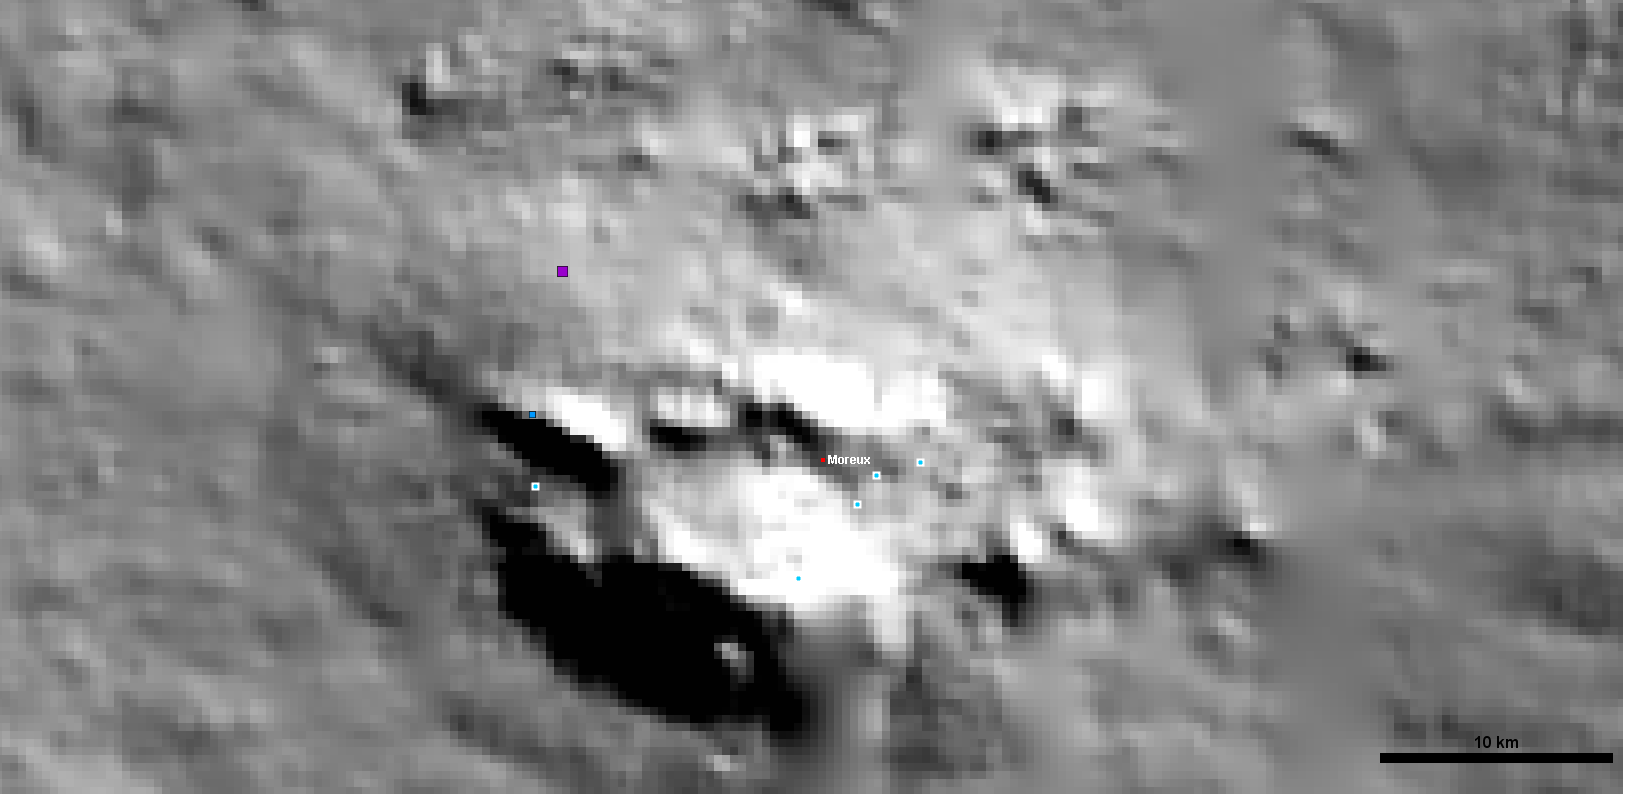
\includegraphics[width=\textwidth]{LandingSite/3_1_3_JMARS.png}
  \caption{Our landing site as shown within JMARS \cite{christensen_engle_anwar_dickenshied_noss_gorelick_weiss-malik_2019}}
\end{figure*}



The science team began landing site selection by splitting Mars into four quadrants, and finding good candidates in each quadrant. The team then met and selected three sites to further analyze. These sites were compared according to each section as shown in figure 3, and the best candidate, Moreux crater, was chosen. Moreux is located just at the edge of potential landing site 53, Protonilus Mensae. The site is located within Unit 2 of Mars, where there is discontinuous shallow ice within 5m of the surface. 

\begin{figure*}
  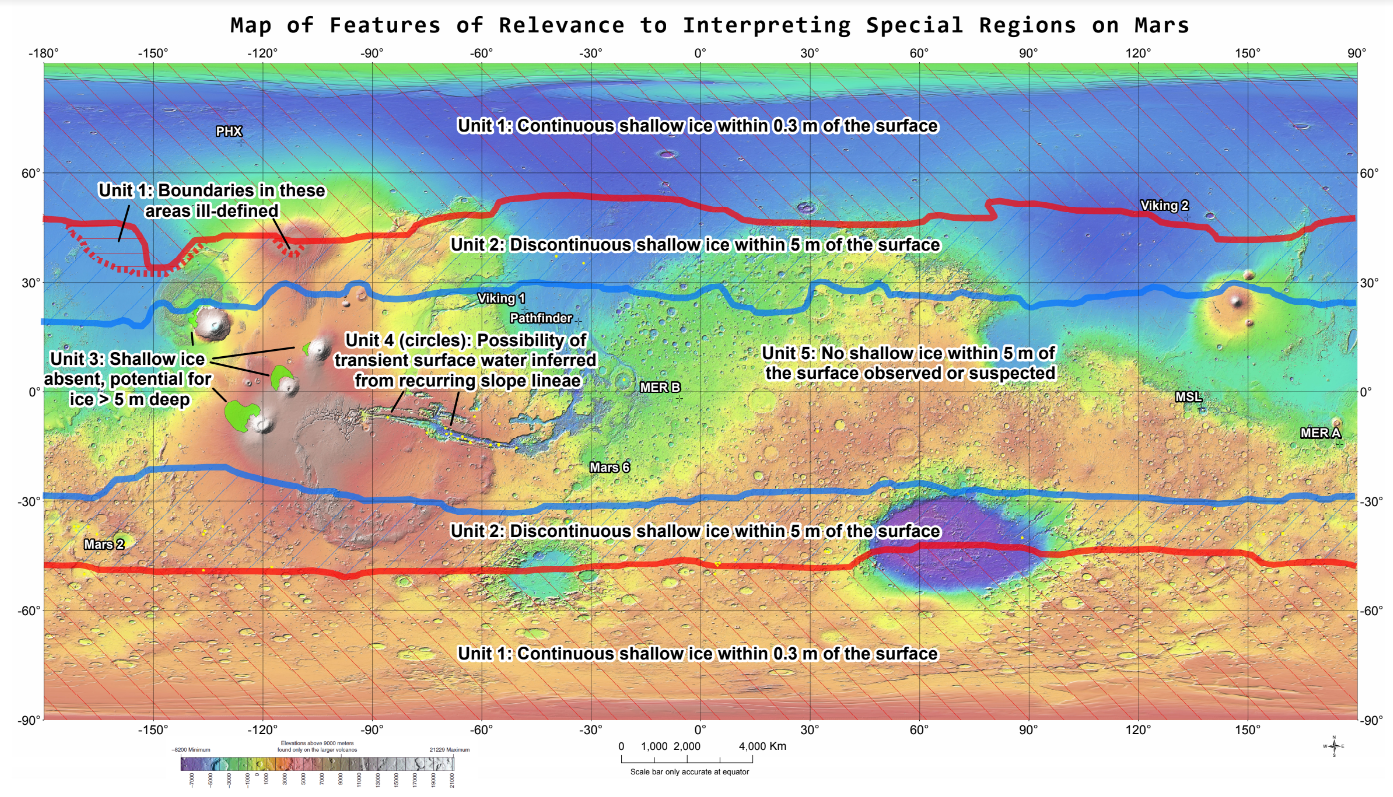
\includegraphics[width=\textwidth]{LandingSite/3_1_3_MarsUnits.png}
  \caption{A map of Mars' special regions}
\end{figure*}

The team has proposed we land directly in the middle of the Moreux crater on top of one of the potential glaciers. There are also hydrated minerals less than 8km from some of the glaciers. Shown in figure 1 are glacier-like forms, indicated by the blue and white squares, and the presence of hydrated minerals, as shown by the purple and darker blue square. According to Sinha and Murty, \begin{quote}
    “We also suggest that central peak of Moreux probably acted as the locus for accumulation of ice/snow and the diversity of glacial/periglacial features within the crater was possibly controlled by differences in the amount of accumulated ice/snow and the rate at which the terrain responded to the shifts in climate during subsequent periods of obliquity changes \cite{sinha2015amazonian}.”
\end{quote}
\begin{figure*}
  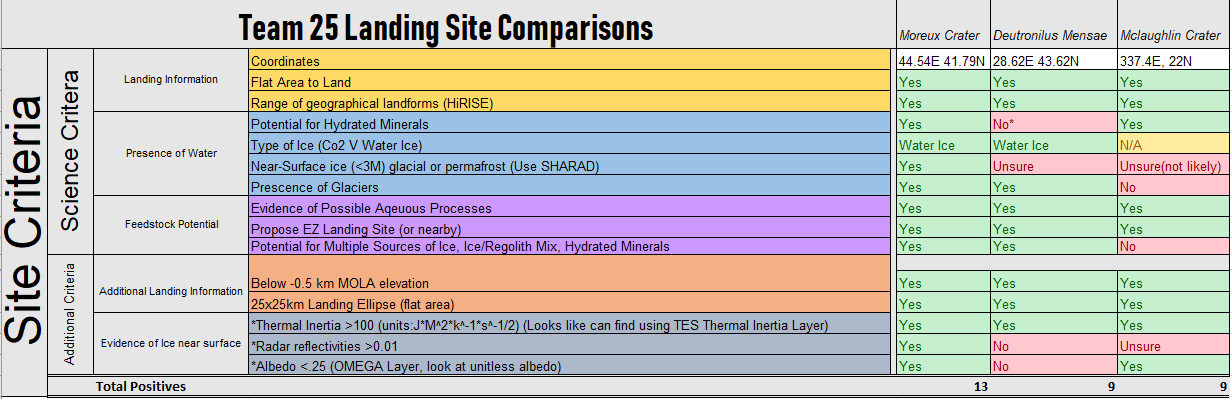
\includegraphics[width=\textwidth]{LandingSite/yLandingSDM.png}
   \caption{Landing site decision matrix}
\end{figure*} 


According to JMARS, the specific location where the mission will take place has the highest chance of surface ice. There is shown there are glacier-like forms at the site, the albedo is less than .25, the Radar reflectivity is less than .01, and the the thermal inertia is less than 100 \cite{christensen_engle_anwar_dickenshied_noss_gorelick_weiss-malik_2019}. All of these point to surface ice to be incredibly likely. 
\\
As for landing at the site, it is well below -.5 km MOLA elevation, the recommended distance for a safe landing, and there is an appropriately wide landing ellipse. The landing site also has high potential for water feed-stock. There are potentially hydrated minerals nearby, and the ice found is very likely to be water ice \cite{christensen_engle_anwar_dickenshied_noss_gorelick_weiss-malik_2019}. 

Assuming a mobile probe, choosing this landing site gives us the ability to sample an area of both hydrated minerals and many glacial sites given the minerals and glaciers are within 10km of each other. A reasonably flat area can be found at the top of the crater shown in figure 1.

%3.1.4
\subsubsection{Describe test and measurement, variables and controls}
It is very important that the instruments work when they land on the surface of Mars. As such, the earth testing process for the instruments must be considered carefully to minimize any unforseen conditions that could arise during the mission. The biggest potential problem is the temperature. The surface of Mars is much, much colder, and there's less atmosphere to retain heat. However, JPL already has a 25 foot wide Mars like testing chamber that could be utilized to ensure the payload is operable under those conditions. A similar proof of concept has already been conducted by a small, autonomous drone that is set to accompany the Mars 2020 rover within this testing chamber \cite{banke_2019}. The payload systems could be tested in this environment. 

To test the APXS, the independent variable would be a mix of CO\begin{math} _2 \end{math} and H\begin{math} _2 \end{math}O. The control group for the experiment would be a pure water sample. The dependant variable will be the readings received from the machine. The independent variable will be changed by adjusting the ratio of CO\begin{math} _2 \end{math} present within the H\begin{math} _2 \end{math}O. A total of six samples will be tested: The control sample of pure water, a sample that is 70\% water, a sample that is roughly 50\% water, a sample that is 70\% carbon dioxide, a sample of pure carbon dioxide, and a sample of water contaminated with martian-like regolith. Things that will need to be controlled for are temperature, air pressure, and gravity. 

%3.1.5
\subsubsection{ Show relevance of expected data, accuracy/error analysis}
APXS has two main ways of taking data, X-rays and alpha particles. Both work through excitation processes. Excitation is where some discrete amount of energy is added to a particle or other system and causes a change in that system, usually causing a change in states (i.e. ground to excited). Simply put, a cross-section is the area where relative to their motion, two particles can interact, collide, and then scatter. As stated in the paper Refined data of Alpha Proton X‐ray Spectrometer Analyses of Soils and Rocks at the Mars Pathfinder Site: Implications for Surface Chemistry, "The cross sections of the excitation reactions depend on energy of the exciting particle and atomic number of the target nucleus. Alpha particle excitation has a high K shell ionization cross section for low Z elements and strongly decreases with increasing Z. For X‐ray excitation, the ionization cross section increases with increasing Z..."
The data taken through the x-ray fluorescence excitation process will be in the form of a x-ray spectra. 
\begin{figure}
  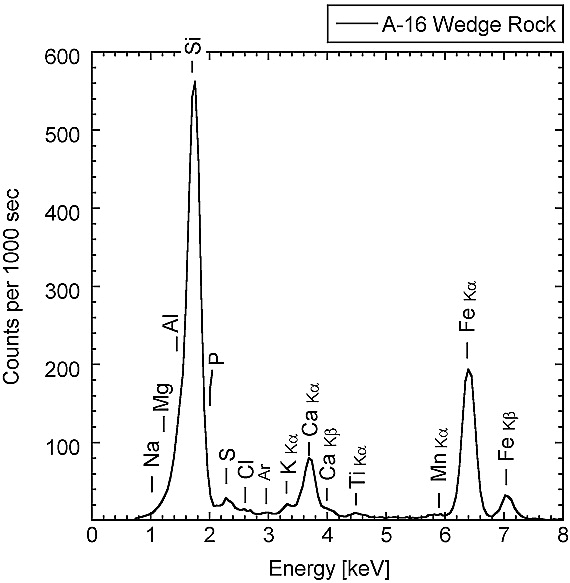
\includegraphics[width=240pt]{Instruments/APXSdata01.png}
   \caption{An example of what APXS data would look like. This sample is a Martian wedge rock \cite{bruckner2003refined}.}
\end{figure} 

\begin{figure}
  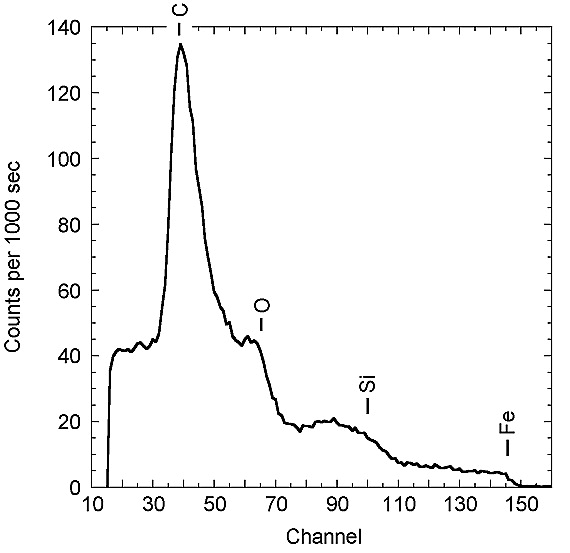
\includegraphics[width=240pt]{Instruments/APXSdata02.png}
   \caption{Second example of APXS data. This is a sample of a different rock \cite{bruckner2003refined}.}
\end{figure} 

The Alpha Spectras of our sample will be of particular interest as the alpha source is particularly sensitive to Oxygen and Carbon. The alpha mode will prove helpful in differentiating if an ice sample is C02 ice or closer to pure H20 ice that could be used as feedstock. 
All other elements will be better determined by using the x-ray mode of the instrument. (An Introduction to the Lunar and Planetary Science Activities in Korea, Advances in Space Research). 

\newpage
There are several elements that will be of particular interest when examining the ice. Perchlorates are one in addition to Chlorine, Lead, Mercury and Arsenic. These elements are toxic to human beings and would be important to identify the presence of in ice that could be a potential future source of water. 
\begin{quote}
    “The average error for each element is derived from the errors of peak areas and calibration curves. The large peaks, i.e., high concentrations, have the smallest errors, while elements that are close to the detection limit of the instrument, show large errors up to 50\% \cite{bruckner2003refined}.” 
\end{quote}
\begin{figure*}
  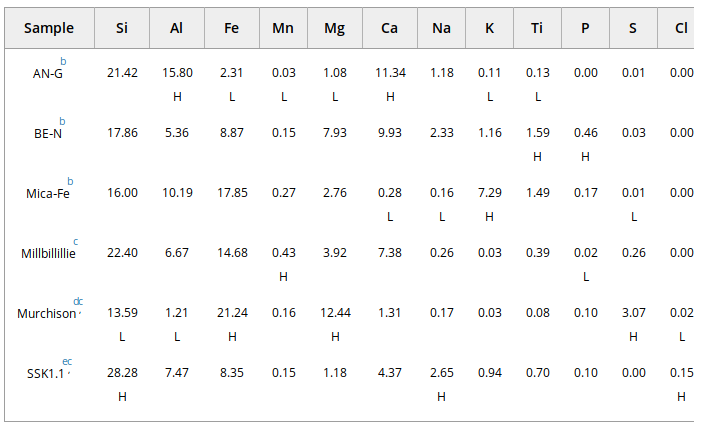
\includegraphics[width=\textwidth]{Instruments/APXSdata03.png}
   \caption{This table shows elemental composition of rock and soil samples taken from Mars with an average error for each element \cite{bruckner2003refined}.}
\end{figure*} 



%3.1.6
\subsubsection{Describe the Preliminary Experiment process procedures}
One of the primary goals of this mission is the chemical characterization of possible ice found at the Moreux Crater landing site. With this goal in mind, preliminary measurements will be conducted on Earth to compare with samples taken on Mars. The APXS instrument will be used with both the X-Ray mode and Alpha mode employed to take measurements. One of the science payload goals is to characterize the ice as being closer to pure water ice or carbon dioxide ice like that found at the poles of Mars. 

The APXS instrument will be used to take sample measurements here on Earth before being sent to Mars. Some samples will be in laboratory conditions and others will be in situ. Laboratory condition samples will include dry ice, deionized water, salt water, frozen deionized water, and frozen salt water. Elements including Chlorine, Lead, Mercury, Arsenic, and some Perchlorates will be added to the water and spectra taken of the water in both liquid and frozen forms. The exact amount of elements put into the water will be at the level toxic to humans. The reason for this is one of the primary goals of our mission is to characterize ice as a potential feedstock option for future crewed Mars missions. In situ sample measurements will be taken of glacial ice in both saltwater and freshwater forms. Possible sites include Antarctica, Greenland, Canada, and Alaska. 
    
Taking on Earth measurements is critical to both test the instrument suite functionality before requiring it to operate in a foreign environment, and generates data to use as a comparison and calibration point for data taken on Mars. Alternate measurements can be taken of data on Earth to ensure the accuracy of taken measurements. Mass spectrometry is one of the methods being investigated to check the accuracy of APXS measurements. 
    
Data taken using the GPR instrument will be taken at the same sites chosen for the APXS instrument. The important feature here is testing the functionality of the instrument on ice that already has a known layer composition. Another goal is to develop image resolution and depth parameters. In other words, how deep of a measurement can be taken and what image resolution is correlated to that depth? One additional goal of this will be to take measurements of areas that have a mix of glacial ice with some other form of terrean. Being able to determine to what level an ice to not-ice ration can be measured will provide valuable information about the possibilities of determining a regolith to ice ratio on Mars. 


%3.1.7
\subsubsection{Describe the steps and procedures the project is taking to integrate communication and planning tasks with the engineering team to optimize the science return}
This project has taken multiple considerations to be sure the engineering team and science team are coordinating together. The first step that was taken was to have a science team liaison to the engineering team. Johnson Seri was a perfect candidate for this position with his experience in physics as well as engineering. The second step taken was to have a weekly meeting for the project manager and team coordinators. The purpose of this meeting was first to develop an agenda for the team's weekly meeting, and second to ensure the engineering and science team were on the same page. Between these two steps, the teams stayed in sync with one another, and should continue to. 

%Begin Section IV
\section{\label{sec:level4}Descent and Lander Criteria}

%4.1
\subsection{Selection, Design, and Verification of Descent and Lander Mechanism}
The driving forces behind the Entry, Descent, and Landing (EDL) system selection were the limitations put on the team by this academy and by Mars itself. With such a small size and weight, conventional landing systems were found to be non-viable. Thrusters to stabilize and perform a soft landing would be too taxing on the weight limitation. So, older NASA missions were looked to for inspiration. In short, the lander will utilize the friction of the atmosphere to slow down significantly, then utilizing a parachute to slow down more. Before touchdown, airbags will be deployed so that the lander may land safely. 
\begin{figure*}
  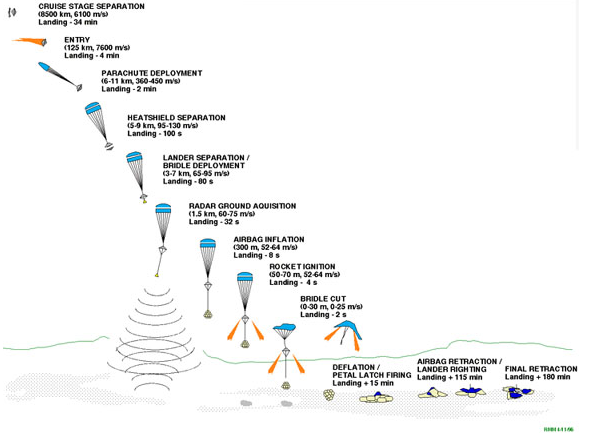
\includegraphics[width=\textwidth]{DescentandLanding/yLandingSequence.png}
   \caption{MER sequence of events, NASA}
\end{figure*} 
Figure 4 shows an example landing very similar in design to this proposed landing.



%4.1.1
\subsubsection{Mission Statement, Requirements, and Mission Success Criteria}

\textbf{Mission Statement:} To successfully and safely land the payload on the target landing site on the surface of Mars, and to successfully obtain surface readings of the planet for the purpose of gathering information for possible water feedstock. 

\textbf{Requirements:} 
\begin{itemize}
	\item A successful descent and landing
	\item The payload operates, and does so for at least three Sols
	\item The payload can successfully communicate back to the buoy, and the buoy transmits back to Earth for data processing
\end{itemize}

\textbf{Mission Success Criteria:} This team must design a machine that will land safely on Mars, and take readings of ice near the surface. This mission will have been a success once the payload has been active and taking readings for three Martian sols. 

%4.1.2
\subsubsection{Major Milestone Schedule}

\textbf{Phase A: Project Initiation}

This phase will include the formulation of the Preliminary Design Review (PDR) as well as laying the foundations for the rest of the mission. Start date: 2/7/2019  End Date: 5/31/2019

\textbf{Phase B: Design}

This phase would consist of refining the mission design continuously until all members of the project are satisfied that the mission has the highest chance of success and will answer all science questions proposed. The Critical Design Review (CDR) would be created and completed in this stage, which becomes the mission's master document for all further stages. Start Date: 6/1/2019 End Date: 5/31/2020

\textbf{Phase C: Manufacturing}

During the manufacturing phase, the actual hardware for the mission is produced. The CDR is followed to produce the mission components to it's specifications. Each element of the lander and payload is manufactured. Any programs or other logic the machine may need would also be written during this time. By the end of this phase, each element will be ready for testing. Start Date: 6/1/2020 End Date: 6/30/2021

\textbf{Phase D: Verification}
This is the testing phase, where each component of the mission will be tested. The Test Readiness Review (TRR) will be written and completed near the beginning of this period, and will conclude when all pieces of the mission are tested thoroughly to work under expected conditions. Start Date: 7/1/2021 End Date: 8/6/2022


\textbf{Phase E: Operations}

This is where the mission launches. This also includes the entirety of the mission flight time. This phase would conclude once the payload has reached its end of life, and all data is collected and prepared for the review stage. Start Date: 8/7/2022 End Date: 4/25/2023

\textbf{Phase F: Major Reviews}

This section consists of reviewing the data received from the mission, analyzing the data, and drawing conclusions from the data. Also included is mission analysis and review. This is where suggestions for improvements and  additions for future, similar missions. Start Date: 4/26/2023 End Date: 9/30/2023

%4.1.3
\subsubsection{Review the design at a system level, going through each system’s
functional requirements}

%(Includes sketches or CAD of options, selection
%rationale, selected concept and characteristics) – all drawings or CAD
%should include a front, side, and top point of view and dimensions of
%each

\textbf{Heat Shield:} The heat shield will protect the lander form the heat buildup of entry into the Martian atmosphere.  Upon entry two small fins at opposite sides of the heat shield will impart a stabilizing rotation to the craft \cite{garber1961analysis}.  Once the craft reaches a reasonable speed the parachute will deploy and the heat shield will no longer be needed.  It will be ejected from the landing craft to reduce the mass and allow for more effective use of the parachute.

The heat shield is a cone with an angle \begin{math} \theta \end{math} that is used to absorb the thermal energy of atmospheric entry.  The material used is for the heat shield is made from tiles of a core of silica fibers with an outer coating made of borosilicate \cite{wiki:001}.  This construction will be similar to the body tiles of the space shuttles thermal protection system.  The thickness of the tiles for the space shuttle were between 12.7cm and 2.5cm \cite{wiki:001}, the thicker ones were located in places were the thermal energy absorption was higher.  Since our lander is less massive than the space shuttle the required thickness will be lower.
\begin{figure}[h!]
  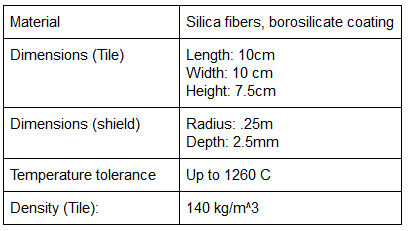
\includegraphics[width=250pt]{DescentandLanding/yHSMatProp.png}
   \caption{Heat shield material properties}
\end{figure} 

When the lander begins its descent the heat shield will absorb most of the thermal energy.  Two small fins will be in position on either side of the heat shield sticking out a short distance.  These fins allow for a .5 to 2 rad rotation per second to stabilize the atmospheric entry vehicle \cite{garber1961analysis}, to keep it from tumbling out of control, as well as evenly distributing the workload across all the heat shield tiles.  The heat shield will allow the lander to decelerate from 6000 m/s to approximately 400 m/s. The parachute will deploy to continue the deceleration.  At this time the heat shield will be detached by explosive bolts \cite{JPL:000}.  The shield will continue down to the planet and land a safe distance away from the lander.

\textbf{Parachute:} After reaching a sufficient velocity the parachute will deploy, slowing down the landing craft further.  Even with the parachute the craft will still be traveling very quickly towards the martian surface.  At a certain distance from the ground small auxiliary boosters will fire slowing the craft down to a new standstill a short distance from the surface \cite{NASAMarsExplorationRovers:002}.  Once the velocity is near zero the parachute will be detached, the craft will fall, and the rockets will carry the parachute a safe distance away.

The parachute will need to be deployed and be able to withstand the forces of slowing down a 7.5kg lander that is traveling with a velocity of around 400 m/s.  In order to do that the parachute needs to be made of very strong, flexible, and light material.  Kevlar is the natural choice.  While materials such as vectran have similar tensile strengths and density, Kevlar has a slightly higher strength and slightly lower density as well as being a more readily available material and therefor cheaper.

The lines connecting the parachute to the lander will be made from Zylon.  Zylon is currently the material of choice for the parachute lines of other EDL landers as well.  It boasts high strength and low mass.  Similar to the latest mars rover, curiosity, the parachute was connected with 48 lines \cite{JPL:002}.  We chose to also go with 48, but the length is somewhat lower to compensate for the mass restrictions of the design.  At 10 meters long and 48 separate suspension lines we are looking at 480 meters of zylon \cite{NASAMarsExplorationRovers:001}.

The auxiliary rockets that will be used to slow the craft down to a final velocity of 0 m/s will be solid fuel rockets to decrease complexity and weight.  They will be using ammonium perchlorate and powdered aluminum for the fuel.  To bring the lander to a stand still we need to apply 833.4 N of force for 2.4 seconds.  By using 3 separate rockets we can ensure stability.  Each rocket is required to be 277.8 N and will fire for 2.4 seconds.  The required fuel will weigh in at .14 Kg.
\begin{figure}[h!]
  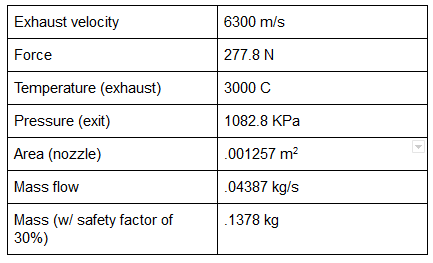
\includegraphics[width=250pt]{DescentandLanding/yauxRocketTB.png}
   \caption{Properties of auxiliary solid fuel rockets}
\end{figure} 

\textbf{Equations:}
\begin{itemize}
    \item \begin{math} Thrust = Force = mV_e + (p_e - p_0)A_e \end{math}
    \item \begin{math} M = pVA \end{math}
    \item \begin{math} P = RT/V \end{math}
    \item \begin{math} F = mA \end{math}
    \item \begin{math} V_2 = v_1 + at \end{math}
    \item \begin{math} \Delta x = V_0t + .5at^2\end{math}
\end{itemize}
All dimensions and properties are as follows \cite{UniversityofIdaho, wiki:004, wiki:005, alqassim2011mechanical, NASAMarsExplorationRovers:001}:
\begin{figure}[h!]
  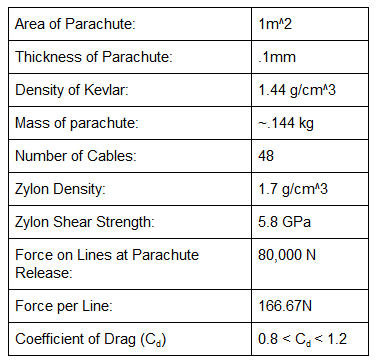
\includegraphics[width=250pt]{DescentandLanding/yParaSpecs.png}
   \caption{Properties of Parachute}
\end{figure} 

\textbf{Equations \cite{wiki:002}:}
\begin{itemize}
    \item \begin{math} Drag = \frac{1}{2}C_dA_ppV^2 \end{math}
    \item Kinematics:
    \begin{itemize}
        \item \begin{math} V_2^2 = V_1^2 + 2a\Delta x \end{math}
        \item \begin{math} \Delta x = v_0t + .5at^2 \end{math}
    \end{itemize}
\end{itemize}

At approximately 10,000m the parachute will be expelled from its housing and will unfurl to slow the lander from 400 m/s to around 200 m/s.  Due to the thin atmosphere further reduction in speed is difficult with parachutes alone.  When the lander gets closer to the surface sensors will detect the distance and at 505m height auxiliary boosters will ignite to bring the lander to a near 0 velocity at around 25-20 m above the surface \cite{NASAMarsExplorationRovers:002}.  Once this is achieved the airbags on the lander will inflate (see airbag section), and the parachute will release the lander.  Once free, the rockets will carry the parachute away so as not to interfere with the lander's mission.
\begin{figure}[h!]
  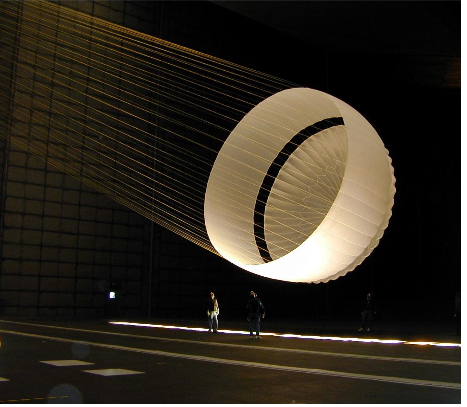
\includegraphics[width=250pt]{DescentandLanding/yexPara.png}
   \caption{Testing of a parachute in wind tunnel, NASA}
\end{figure} 

\textbf{Lander Craft Construction:} When the craft is coming to a standstill a few tens of meters off the surface the landing craft will inflate air-bags on all sides of the craft before detaching from the parachute.  The craft will freefall to the surface and the airbags will absorb most of the energy.  Once the landing craft comes to a stop the airbags will slowly deflate due to the pressure imbalance.  When that is complete one door will open at a time.  With the pyramidal shape of the craft we can guarantee that the craft will not end up upside down and unable to open.  If it is on its side, the opening of the shell will flip the craft right side up.  When all sides are open the lander can carry out its mission.
\begin{figure}[h!]
  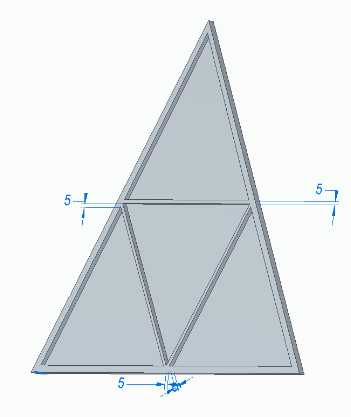
\includegraphics[width=250pt]{DescentandLanding/LandingCraftSide.png}
   \caption{One side of the lander with supports shown}
\end{figure} 


The support structure of the lander consists of 2cm x 2cm honeycomb aluminum.  This allows for high strength and low mass.  All together the volume of the support will be .0048 m\begin{math}^3 \end{math}, and with a density of between 163 kg/m\begin{math}^3 \end{math} and 20 kg/m\begin{math}^3 \end{math} (we used the 163 kg/m\begin{math}^3 \end{math} for calculations) we end up with a total mass for the super structure of .7824 Kg.  Between the superstructure and the airbags there is an insulating backing of aluminum foil totaling .1mm thick.  Spanning 2 m\begin{math}^2 \end{math}, and a density of 2.7 g/cm\begin{math}^3 \end{math} we end up with a total mass of .2 Kg.  With all these in place the superstructure will be able to take a beating.
\begin{figure}[h!]
  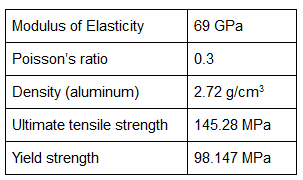
\includegraphics[width=250pt]{DescentandLanding/LanderTable.png}
   \caption{Properties of Lander}
\end{figure} 
\begin{figure}[h!]
  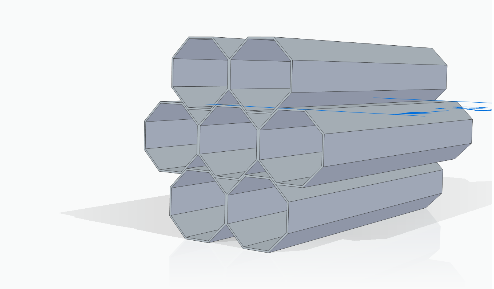
\includegraphics[width=250pt]{DescentandLanding/HoneyCombSupports.png}
   \caption{Example of the honeycomb supports}
\end{figure} 
The landing craft is the housing that contains the lander.  Its job is to get the lander onto the surface of mars in working condition.  The landing craft is comprised of multiple systems; The parachute, the airbags, the heat shield, and the lander shell.  The system as a whole is designed to get the lander from the top of the martian atmosphere to the surface safely.  The shell is comprised of three triangular doors, the floor panel, and all supporting electrical equipment (heating elements, motors, sensors).  The fame of the landing craft will support the parachute housing, as well as the housing for the airbags.  The skeleton of the structure will be made with honeycomb aluminum to maximize strength and minimize density \cite{zylonByToyobo}.

On the inside of each of the three doors there is an electric motor to open the doors upon landing.  If the lander lands right side up then the doors will be opened one at a time.  If the lander ends up on its side then a sensor will let the lander know what side is currently face down and will open that door first.  When it opens it will push the landing craft over so that the lander is right side up.  Then the opening of the landing craft will continue as before. 


%4.1.4
\subsubsection{Describe any subsystems that are required to accomplish the overall mission}
The lander does have one critical subsystem: the airbags. The airbags are designed to absorb the kinetic impact of the lander impacting the surface.  Upon inflation the airbag system will maintain a constant 6.895 kPa (1 psi).  Once the lander finally stops, the airbags will slowly deflate and after 90 minutes we can assume that the airbags are fully deflated.  At that time, the first side will open and if the rover is on its side the side will flip it right side up easily due to the pyramidal shape of the lander.  Once all 3 sides are open the lander will be free to focus on its mission. 
\begin{figure}[htp]
  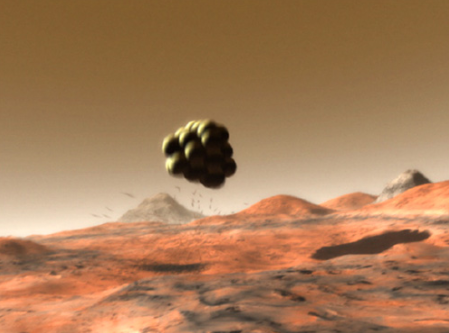
\includegraphics[width=240pt]{DescentandLanding/PFairbagRender.png}
   \caption{Pathfinder airbag render, NASA}
\end{figure} 

The gas that will be used is similar to what is used in automobile airbags.  WIth high chemical stability and reliability Sodium Azide (\begin{math}NaN_3\end{math}) is a good choice.  Upon heating \begin{math}NaN_3\end{math} the molecule readily decomposes into Na and N (see stoichiometric equation in table).  The Nitrogen gas fills the airbags to a pressure of 6.895 kPa, approximately 1 psi, allowing a soft landing upon the martian surface.  The approximate volume of one air bag is calculated to be \begin{math} .0625 m^3 \end{math}, and being a four sided pyramid we have four airbags with a total volume of \begin{math} .25m^3 \end{math}.  To achieve a volume of gas at that size we need .826 moles of sodium azide.  However we will also have some small vents to allow for the gas to escape upon landing.  These vents will be approximately \begin{math} 8cm^2 \end{math}, there will also be an effusion rate of approximately \begin{math} 1.225*10^{-6} \end{math}moles/sec.  To make up for the effusion of the gas and loss from the impact we will include enough of the sodium azide to make \begin{math} .5 m^3 \end{math}  of \begin{math} N_2 \end{math} gas.  1.652 moles weighing in at 107.4g will be required.

The airbag material themselves will be made out of kevlar, boasting high strength and low density it is the best choice \cite{JPL:001}.  The surface area of the bags is 5.2 \begin{math} m^2 \end{math}, with a density of \begin{math}  114g/m^2\end{math}, weighing in at .6 kg.  They will be folded up and sealed with a quick release band to allow for fast inflation.
\begin{figure}[h!]
  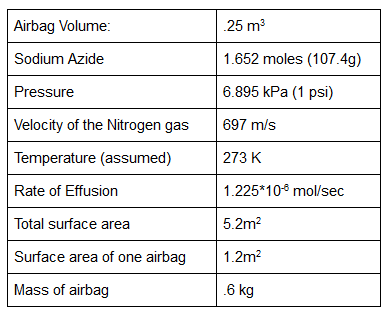
\includegraphics[width=240pt]{DescentandLanding/airbagSpecs.png}
   \caption{Properties of airbags \cite{wiki:005}}
\end{figure} 

The expressed purpose of the airbags is to get the lander safely onto the surface.  Once the parachute and auxiliary rockets slow the lander down to 0 m/s at around 25m above the ground the parachute will be detached and flown away to a safe distance and at the same time the gas generators will heat the sodium azide, inflating the airbags \cite{NASAMarsExplorationRovers:002}.  Upon full inflation the gas generators will maintain a minimum of 1 psi in the air bags \cite{JPL:000}.  When the lander impacts the ground the force will be dampened by the airbag.  Once the lander has come to a complete stop the gas generators will continue to keep the pressure at 1 psi, but will eventually run out of fuel and then the gas will effuse until the pressure within the bags is equal to the pressure of the atmosphere.  We will wait 90 minutes to allow for the equalization.  Once that time passes we can move on to opening the landing crafts doors.

The required subsystems would include all the computer system required to control the stabilization fins of the heat shield.  The rangefinder on the lander that will let the craft know how far above the surface it is.  The triggering system to release the heat shield.  The control system for the airbag  inflation and pressure regulation.  The control and release system for the parachute.  The wiring harness to connect all the different systems together.

%4.1.5
\subsubsection{Describe the performance characteristics for the system and subsystem (if applicable) and determine the evaluation and verification metrics}
Each of the systems have a pass or fail status, since the specifications of the mission don’t allow for much in the terms of backups in case of any failures.  If the door does not open, the mission is a failure.  If the parachute does not deploy, the lander will crater into mars and the mission is a failure.  If one of the three bolts do not shear off properly, the parachute will not be able to slow the lander down enough and the mission will fail.  Everything will need to go according to plan the first time.

Each of the components of the subsystems need to be tested and make sure that they can function with a safety factor to give a little wiggle room in case something is slightly off.  For example, if the lander ends up on its side the the motor must be able to create a moment sufficient to flip the lander right side up to allow for the rover to complete its mission.  Creating a rubric for exactly what each system and subsystem needs to do is important.  If any piece of equipment can not accomplish that, then the design needs to be reworked until the subsystem can accomplish the mission.

\begin{figure*}
  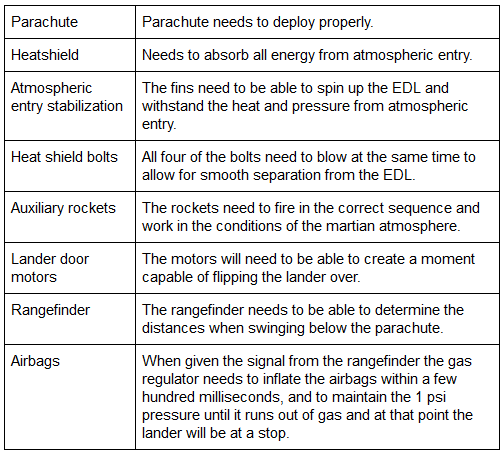
\includegraphics[width=\textwidth]{DescentandLanding/4_1_5.png}
   \caption{Verification metric for descent and lander system}
\end{figure*} 

%4.1.6
\subsubsection{Describe the verification plan and its status}
Upon clearing all testing procedures we can certify that all the systems and subsystems can meet and exceed all the hazards and challenges that the lander will meet.  We have set a bar of a safety factor of 30\%. This means that the lander is designed to exceed the requirements of landing safely on Mars by 30\%. By creating the subsystems to exceed the minimum requirements we can safely say that if the subsystems do not outright fail that they will be able to do their job.

%4.1.7
\subsubsection{Define the risks and the plans for reducing the risks through analysis or
testing for each system. A risk plot that clearly portrays the risk
mitigation schedule is highly encouraged.}
Every part of the EDL system will be tested in situations that simulate the environment that the lander will experience en route and on Mars.  We will test prototypes of the lander in testing chambers that can mimic the conditions that the lander will encounter such as the vacuum of space, the vibration and forces exerted on the lander during launch, dust from the landing itself, the heat from atmospheric entry.  

%4.1.8
\subsubsection{Demonstrate an understanding of all components needed to complete
the project and how risks/delays impact the project}
The main systems required to get the lander on the ground are; The heat shield system, the parachute system, the airbag system.  With these main systems we also have sub systems such as for the parachute system.  It needs the rangefinder in order to know when to ignite the auxiliary rockets to bring the lander to a stop 25 meters above the ground.

%4.1.9
\subsubsection{Demonstrate planning of manufacturing, verification, integration, and operations. (Include component testing, functional testing, or static testing)}
Due to the nature of the constraints, mainly monetary, most parts will be cheap, easy, and readily available.  Micro-controllers such as raspberry pi, and Arduinos will be used when their specifications will suffice.  Extra shielding will be needed to allow the controllers to work in a vacuum and on the near vacuum of the martian surface.  Other materials such as the Kevlar of the parachute are mass produced with a high level of quality.  For the aluminum honeycomb we will use metal deposition 3D printing to create the intricate design of the honeycomb that allows the strength benefits of the aluminum with the weight cutting benefits of the honeycomb structure.

All the components that go into building the EDL system will be testing for functionality upon receiving the parts.  Micro-controllers will be placed, similar to the prototype, in testing chambers that will mimic the conditions of space and the martian surface.  They will be tested to make sure that they can do what they were designed to do such as the rangefinder being able to track distances and to trigger an event when a certain distance is detected.

%4.1.10
\subsubsection{Confidence and maturity of design}
The main technologies of the EDL system are tried and true technologies that have been used to success in the past.  Both Viking missions, Pathfinder lander, and the \textit{inSight} lander all used the heat shield into parachute, into airbag landing technique.  There are few other ways to get a small rover onto the surface of Mars, but they require super sonic retro rockets.  The problem with that, is rockets require fuel, and fuel is heavy.  With the parameter of 5 kg, there is just no way to land a capable rover on the ground using rockets.

Combining many different techniques together we can lower the mass of all the systems and create overlapping  ways of slowing the descent of the lander.  The parachute works well at medium velocities, the heat shield works well at high velocities, and the airbags work well at low velocities.  Using all three gets the lander onto the surface safely.  If we tried to use only one or two techniques the mass would explode due to the nature of the atmosphere being so low.

The setup we chose has been proven over decades and many missions, it is the best bet in terms of success rate as well as the best track record for successful missions.  We will add to the success rate.


%4.1.11
\subsubsection{Include a dimensional CAD drawing of entire assembly}
See figures 18, 19, and 20.
\begin{figure*}
  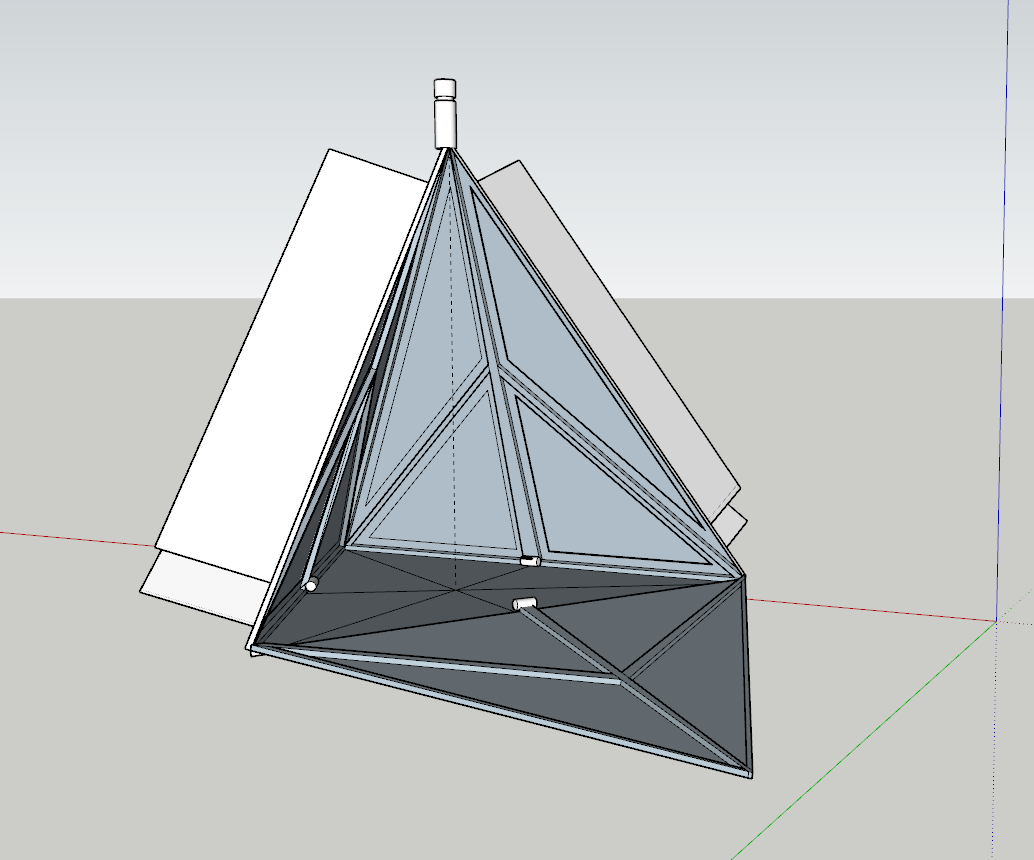
\includegraphics[width=400pt]{DescentandLanding/whol_thing.png}
   \caption{EDL full assembly angle 1}
\end{figure*} 
\begin{figure}
  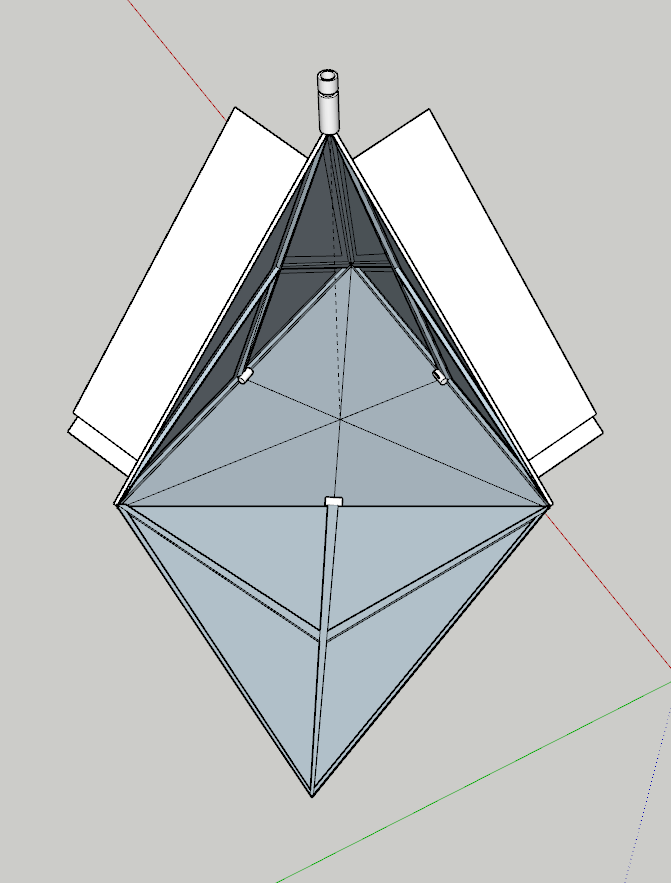
\includegraphics[width=240pt]{DescentandLanding/while_thing_2nd_angle.png}
   \caption{EDL full assembly angle 2}
\end{figure} 
\begin{figure}
  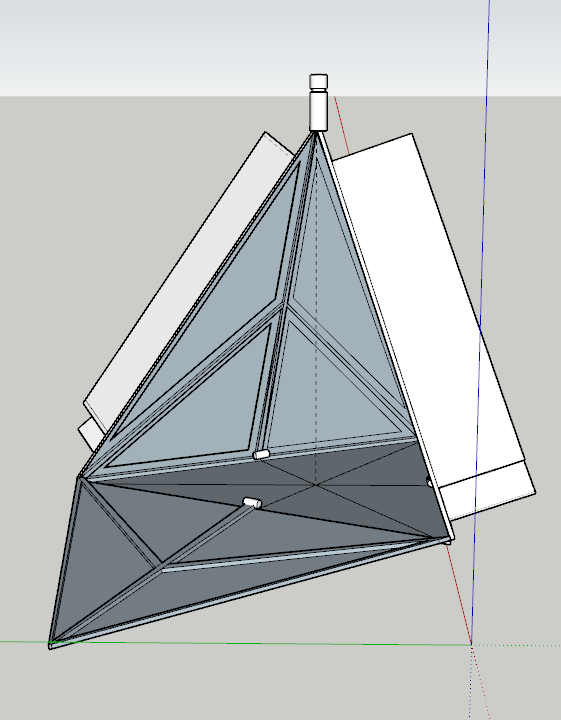
\includegraphics[width=240pt]{DescentandLanding/whole_thing_angle_3.png}
   \caption{EDL full assembly angle 3}
\end{figure} 

%Section 4.2
\subsection{Mission Performance Predictions (Critical)}

%4.2.1
\subsubsection{State mission performance criteria}
As with all missions we expect everything to go according to plan.  With proper preparation, testing, and safety factors the mission should be a success.  The EDL will safely bring the rover from space onto the mars surface.  The heat shield will prevent the lander from burning up.  The parachute will keep the lander form cratering into the surface.  The airbag will cushion the landing for the rover.  The lander will make sure the rover is on its feet.  And the Rover will carry out its mission of finding water on Mars, giving us crucial information needed when planning the next step; A human mission to the red planet. 


%4.2.3
\subsubsection{Show flight profile simulations, altitude predictions with simulated descent and lander data, component weights, and different descent profiles depending on Mars local weather conditions at the team’s choice of a landing site}
A python library, the Python Astrodynamics Project, would be used to model the flight profile for this mission. The package is fairly well developed and robust, but it would have to be reviewed in depth to see if it would encompass all of the mission's needs. This could be a very good opportunity to offer research funds to institutions to test and build up this software. 

%4.2.4
\subsubsection{Show Stability margin, simulated CP: Center of Pressure/ CG: Center of Gravity relationship and locations}
See above section, 4.2.3.

%Section 4.3
\subsection{Payload Integration}

%4.3.1
\subsubsection{Describe Integration plan with the Mars Orbiter and the probe payload}
Integration onto the orbiter will be accomplished by using the parachute housing as the attach point.  The parachute assembly is connected directly to the load bearing support structure of the lander so this will make a good place to connect.  On the housing there will be a grove cutout that will allow for a holding mechanism to grab a hold and connect it to the orbiters side.  When deployment is scheduled the orbiter will rotate to the proper angle and will send the ELD vehicle on its way to the martian surface.

%Section 4.4
\subsection{Earth Testing Operation Procedures}

%4.4.1
\subsubsection{Determine what type of testing system will be used for the Earth analog testing of a component of your science experiment}
\textbf{Heat Shield:} For testing of the heat shields thermal dissipation efficiency we would insert it into a testing apparatus in which one side is heated up to a temp that the heat shield tile would experience during entry of the martian atmosphere.  This would allow us to fine tune the exact thickness required to keep the lander from thermal damage.

For testing the aerodynamic properties of the shape of the heat shield we can place it within a wind tunnel to study how the flow if affected by the angle of the heat shield, how the fins will function under the atmospheric entry conditions, and the rotation needed to stabilize entry.  Below are the Reynolds numbers for different elevations and the air density of the martian atmosphere.  Using the Reynolds numbers we can accurately test the aerodynamic properties without needing to create a wind tunnel that has 6000 m/s and a density of \begin{math} 1.2*10^{-5}  kg/m^3 \end{math}.
\begin{figure*}
  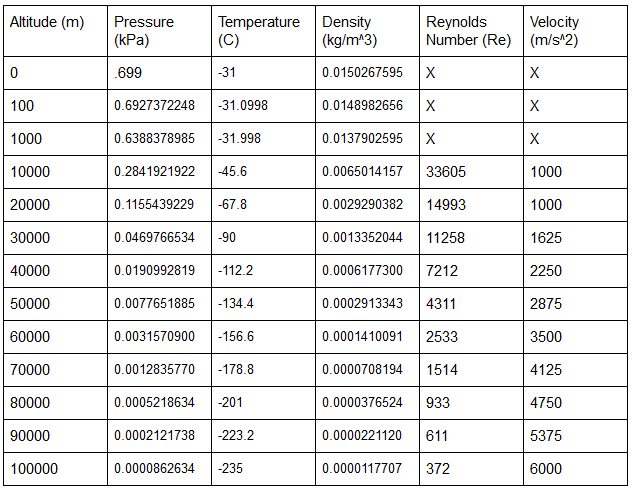
\includegraphics[width=\textwidth]{DescentandLanding/4_4_1_HeatShield.png}
   \caption{Heat Shield testing table. Values at \begin{math}<\end{math}1000 meters not calculated due to unknown velocity \cite{wiki:003, NASA, wiki:005}.}
\end{figure*} 
Some assumptions must be made in light of incomplete information. These are: 
\begin{itemize}
    \item Velocity will decrease at 625 m/s per 10,000 m for simplicity
    \item Thickness for entire heat shield was 7.6cm
    \item Coefficient of Drag is \begin{math} .8 < Cd < 1.2 \end{math}
\end{itemize}
Equations:
\begin{itemize}
    \item Re = \begin{math} \frac{pVD}{\mu} \end{math}
    \item Atmospheric density = P/gh
    \item Temperature below 7000 meters = \begin{math} -31 -(9.98*10^{-5})h \end{math}
    \item Temperature above 7000 meters = \begin{math} -23.4 -(2.22*10^{-3})h \end{math}
    \item Pressure = \begin{math} .699e^{(-.0009(h))^7} \end{math}
\end{itemize}

\textbf{Parachute: } Testing will consist of placing the prototype parachute in a wind tunnel to test that its material strength will hold up in a real world situation.  By determining the Reynolds numbers for various speeds and atmospheric density we can test all the different condition that will occur on mars.  With the reynolds number we can use more dense air at a lower velocity.  This may result in being able to use a more affordable wind tunnel; by using air at lower speeds we can simulate less dense atmosphere at high velocities.  At the max velocity of 1000 m/s, which occurs at 10,000 meters, the Reynolds number is 33605.

We can also use the prototypes to test out the different ways of packing the parachute into its housing.  We may be able to find an efficient way to pack it that allows for a very high chance that the parachute will deploy without tearing.

\textbf{Landing Craft: } Testing of the landing craft itself will consists of dropping the craft to test for any structural failures.  By design the craft will be dropped from approximately 15 - 25 meters above the martian surface and will impact with a velocity of around 10 to 14 m/s.  The structure will need to be able to survive the initial impact and probable resulting bounces.  With a martian gravity equal to about \begin{math} \frac{1}{3} \end{math}of earth's gravity (g mars = \begin{math}3.711 m/s^2\end{math}) the maximum height required to achieve 14 m/s on earth is 10 meters.  Easily achievable at a testing facility.  One hopes to land on a flat barren surface free of debris, but things rarely work out so we will need to test with rocks and terrain deformations.  Adding these to the landing zone in the test area can reveal weaknesses in the design that we can fix.

A big issue is how the craft will function as a whole after being exposed to the frigid temperatures of space.  To make sure that all electronics, materials, and chemicals will function as expected the landing craft will need to be placed in a vacuum chamber and the temperature lowered to -235 C to simulate space like conditions.  If any systems do not perform within specifications then they need to be changed so that they do.

\textbf{Airbags: }Testing of the airbags will consists of making sure that the amount of gas available will be sufficient.  This can be accomplished at the same time as the testing of the strength of the airbag skin.  Taking into account the lower gravity of mars we do not need to drop it from the same height.  Running the kinematic equations we get that the needed height on earth is only 10 meters.  By dropping from that height we simulate dropping from about 25 meters on mars \cite{JPL:000}. We can change the area of landing by manipulating the gradient of the ground as well as introducing obstacles that may occur on the martian surface such as large boulders.  By creating the worst case scenarios we can make sure that the lander can survive and accomplish the mission.



%4.4.2
\subsubsection{Develop an outline of final assembly for the Earth testing}
Final assembly will be the rover installed and secured within the lander housing.  The doors of the lander will be secured shut with the parachute housing holding them closed.  The 4 sides of the lander will have the airbag system secured with a quick release strap for when the gas is released.  The parachute will be packed away in the housing with the release mechanism.  Finally the heat shield will be bolted on with the explosive bolts primed and ready to go off when the lander is ready to deploy the parachute.

%Section 4.5
\subsection{Safety and Environment for Protocols for Earth-based Testing of a Component from Your Science Experiment}
Testing procedures will have a safety officer on site to make sure that all safety rules are followed.  For all testing of the mechanical properties of the lander work areas will be clear of debris, staff will be a safe distance from the actual testing area, proper eye-wear will be work in the worst case if something flies at a testers face, and if something goes wrong (such as a misfiring of the explosive bolts of the heat shield) we will require a sufficient time will need to pass before the researchers will be allowed to approach the prototype.  In the event of a break when testing the support structure of the lander and there are sharp edges, foam caps will be placed over the ends to prevent lacerations.  Any heavy equipment will either be carried by a team of people or if very heavy, a forklift or other applicable heavy machinery will be used to transport the lander.

For the electrical portions, if a technician is working on the electrical parts they will have a ground strap at all time to prevent static electricity from building up and damaging the parts.  If there are any high voltage work that will occur, such as the solar panels, proper protective equipment will  be required (rubber gloves).  


%4.5.1
\subsubsection{Identify Safety Officer for your team (must be present in-person at
Earth testing site or Team Safety Officer need to designate an on-site person.)}
This team's safety officer is Bridgette Davey. She has proven a valuable member of the team and, as telecommincator, is already responsible for contacting team members when needed. 

%4.5.2
\subsubsection{Provide a Preliminary analysis of the failure modes of the proposed design of the descent and lander vehicles, payload integration and deployment
operations, including proposed and completed mitigation}
Failures are as follows:
\begin{itemize}
    \item Parachute does not deploy/lines tangled
    \item Heat shield fails to separate
    \item Heat shield tiles fail
    \item Rangefinder is blocked/does not work
    \item Airbags do not deploy
    \item Auxiliary rockets do not fire/move the parachute out of the way
    \item Support structure failure
    \item Stabilization of atmospheric entry is chaotic
    \item Failure of electrical components
    \item Lander door does not open
    \item Lander craters due to something unforeseen
\end{itemize}
Because of the limitations on weight and space backup systems are not feasible for all points of failure.  For some small electrical components such as the rangefinder backups are possible but a backup airbag system is out of the question.  Because of the low cost of the project multiple missions can be sent out and if a few fail it is not a big loss, the landers are designed with a simple job in mind; Find out if there is drinkable water in the immediate vicinity.  

%4.5.3
\subsubsection{Provide a listing of personnel hazards}
Hazards will include: 
\begin{itemize}
    \item Electrical currents, for electrical components
    \item Explosive hazards from the explosive bolts for the heat shield separation
    \item Chemical hazards from the airbag gases
    \item Sharp edges of the lander
    \item Pinching hazards, does not seem hazardous but still hurts
\end{itemize}
For brevity's sake, the required Material Safety and Data sheets are included in the appendix, under \cite{fisher_scientific_2014, new_jersey_department_of_health_2013, fisher_scientific_2014_001, nuplex_2013}. They will also be included in Appendix C.

%4.5.4
\subsubsection{Discuss any environmental concerns – Explain optimal testing
environment conditions (e.g., weather conditions, landing surface, etc.)}
Because the lander is designed to operate with the atmosphere of Mars and the vacuum of space the EDL is not designed to deal with moisture.  No testing should be done in the rain or extremely moist areas.  If  extreme moisture is a condition testing should be placed on hold or taken into a building with a robust climate control system.

The chemicals involved with the EDL should only be worked with in a well ventilated work space or in an outside testing area.  For the RDX explosives in the explosive bolts, utmost caution needs to be taken.  While the actual explosive is quite small, it can still take off fingers and flying debris can damage soft tissues such as the eyes.  Proper safety equipment needs to be worn.


%Begin Section V
\section{\label{sec:level5}Payload Criteria}

%5.1
\subsection{Selection, Design, and Verification of Payload Experiment}

%5.1.1
\subsubsection{Review the design at a system level, going through each system’s
functional requirements}
\textbf{Selection Rationale:} Once again, the driving force behind this team's selection rationale is the small weight requirement. Several payload instruments were considered, but a large majority were simply too heavy. The most promising of instruments that were not selected was a Palm Portable Mass Spectrometer (PPMS), shown in figure 22. 
\begin{figure}[h!]
  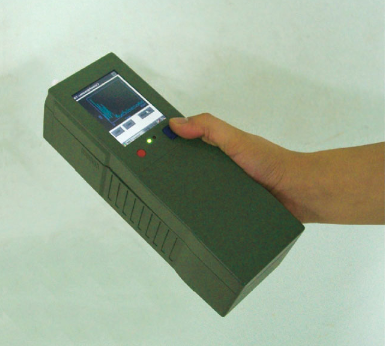
\includegraphics[width=240pt]{Instruments/5_1_1_PPMS.png}
   \caption{A fully assembled PPMS \cite{yang2008development}}
\end{figure} 
Unfortunately, the total weight needed for the PPMS to function correctly was about 1.48 kg, and this did not include any sort of drill that would've been needed; the lightest of which that was found was heavier than our total weight allotment. It was decided to go for lighter alternatives detailed below. 

\textbf{APXS: }APXS or alpha particle x-ray spectrometer is an instrument our probe will inherit from previous mars exploration rovers: Spirit, Opportunity, and Sojourner. The APXS instrument’s function will be to relay information about the chemical composition of glacial regolith mixture at our Probe’s landing sites. There are two main types of radiation APXS will use, alpha particles and x-ray waves. The methods for determining the elemental chemistry of the sample are Particle Induced X-Ray Emission and X-Ray Fluorescence. A Curium-244 source is used for the X-Ray spectroscopy. This instrument's head is only a mere 52 mm wide and 88 mm long. The overall weight is only .6 kg, and the power draw .4 W \cite{bruckner2003refined}. 

\begin{figure}[h!]
  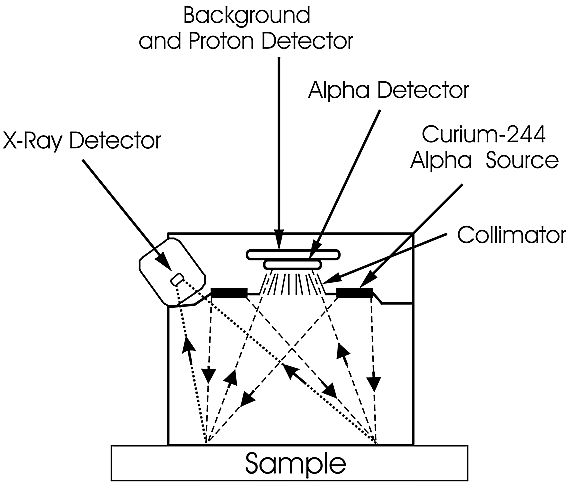
\includegraphics[width=250pt]{Instruments/xAPXS.png}
   \caption{APXS instrument diagram \cite{bruckner2003refined}}
\end{figure} 

When the sensor is pressed up against a sample, in order to get a good reading, the distance between the sensor and the sample must be less than 2 cm. The ideal sample size is 1.7cm in diameter. Depending on the caliber of data desired, the data can be taken anywhere from 10 minutes to a more complete spectrum at 3 hours. The produced data set will be 32kb and produce 13 spectra \cite{APXSspaceflight101}. The X-Ray detector chip should function at temperatures beneath zero degrees celsius, because of this requirement it will only be operated at night when the temperatures on Mars are beneath this. 

The primary function of the APXS instrument will be to determine if the ice it is sampling is CO2 or H2O ice. In particular, the backscattered alpha spectra will provide additional data on the possible presence of Carbon and Oxygen in the ice sample \cite{rieder2003new}. The X-Ray spectra will give information on a wide range of elements from Sodium up through Yttrium. Checking for levels of contaminants or elements that may make the ice unsafe for human consumption is another area of interest to which the APXS will be applied. In addition, the APXS instrument will be used to create a rough estimate of the regolith to ice ratio. If it is within reach of the Probe, APXS can also provide information on any hydrated minerals present at the landing site. 
\begin{figure}[h!]
  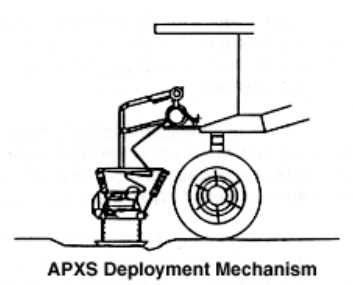
\includegraphics[width=250pt]{Instruments/5_1_1_APXSDeployment.png}
   \caption{APXS deployment mechanism \cite{APXSdescription}}
\end{figure} 

The instrument will be callibrated to be sensitive to sulphur, "As most rocks do not contain much sulphur," it can be used as a measurement of how much soil was detected by the instrument, obscuring the sample. Martian soil has a high concentration of sulphur, so this should be a reliable measurement \cite{bruckner2003refined}.

\textbf{MGPR: }The Mini Ground Penetrating Radar, or MGPR, is a lightweight miniaturized radar that will serve to help identify the quantity of ice present at the landing site. MGPR will also serve to characterize the homogeneity of the layers beneath it at distances up to 50 meters. The ground penetrating radar has a fairly moderate resolution of 1.5m.  At shorter distances of up to 5m, the GPR has an increased resolution of 15cm. This increased resolution can provide valuable information about the ice to regolith ratio and the future accessibility of ice for feedstock in crewed Mars missions. MGPR can also give further information about landforms in the Moreux Crater that illustrate the history of glacial movement. 

The radar works by emitting electromagnetic waves from an EM wave source that are sent into the ground. When the signals encounter a change in the subsurface, they are then reflected back and picked up by a receiver antenna. Changes in the waves represent either a change in the composition of the material sampled or a change in the depth of the subsurface material. Information pulled from the amplitude and wavelength of the waves can give insight into the porosity, dielectric properties, density, and water content of the sampled area \cite{kim2012miniature, conyers2006innovative}. 
The instrument consists of 2 boards 5 cm wide, 10 cm long, and 2 cm tall. It weighs a total of .045 kg and draws 1 W of power \cite{kim2012miniature}. 
\begin{figure}[h!]
  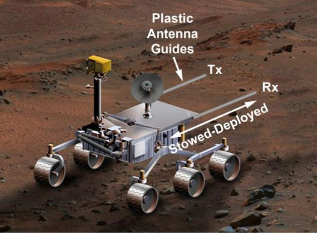
\includegraphics[width=250pt]{Instruments/xMGPR.png}
   \caption{Mini Ground Penetrating Radar on example rover \cite{kim2012miniature}}
\end{figure} 

The MPGR is a fantastic addition to the payload instrument suite. It provides higher resolution readings than a traditional orbital based ground penetrating radar (GPR), as shown in figure 26, and it is extremely light. 
\begin{figure}[h!]
  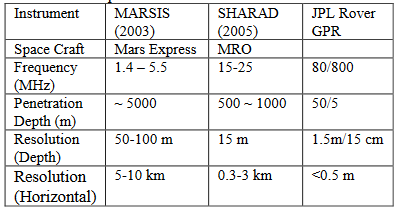
\includegraphics[width=250pt]{Instruments/5_1_1_MGPRcompare.png}
   \caption{MGPR in comparison to orbital GPRs \cite{kim2012miniature}}
\end{figure} 

 In addition to the scientific value of the readings obtained by this instrument, it may also allow the payload to maneuver to a location where ice is more readily available, in the event the payload does not land on one. As the instrument can detect water ice to a depth of 50/5 m, it provides a fail-safe in a mission where there is little room for error.
\begin{figure*}
  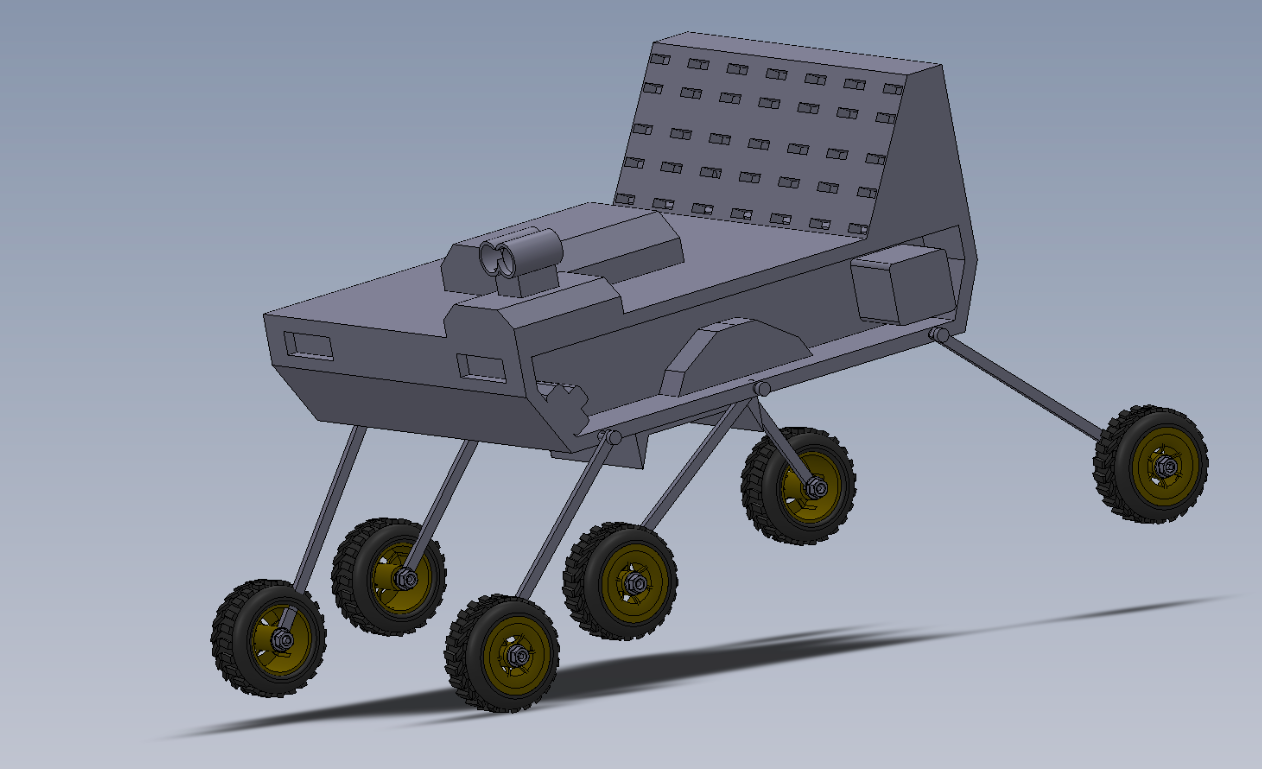
\includegraphics[width=300pt]{Instruments/roverAngle1.png}
   \caption{The 1st angle of the rover's CAD model}
\end{figure*} 
\begin{figure}
  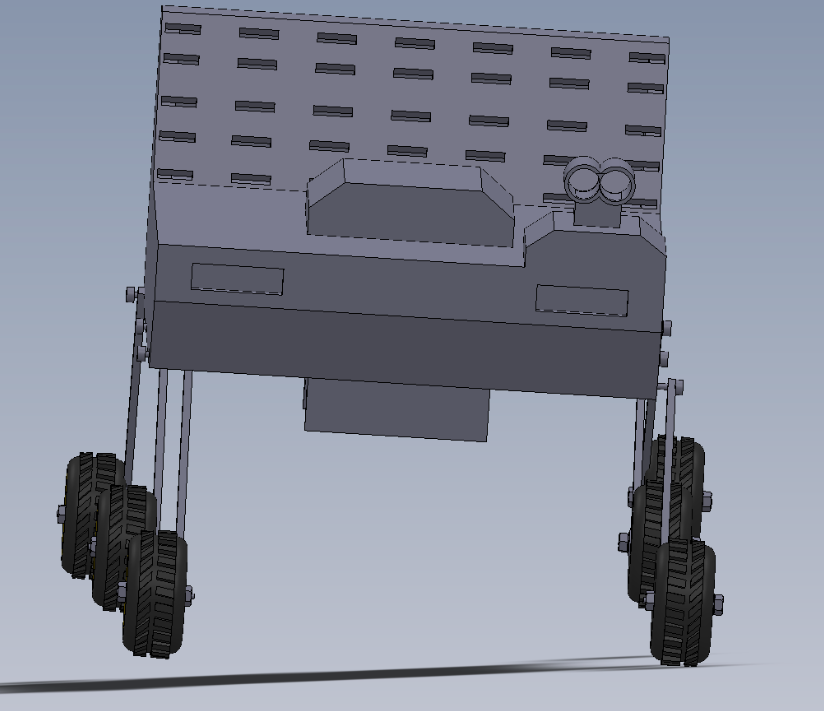
\includegraphics[width=240pt]{Instruments/roverAngle2.png}
   \caption{The 2nd angle of the rover's CAD model}
\end{figure} 
\begin{figure}
  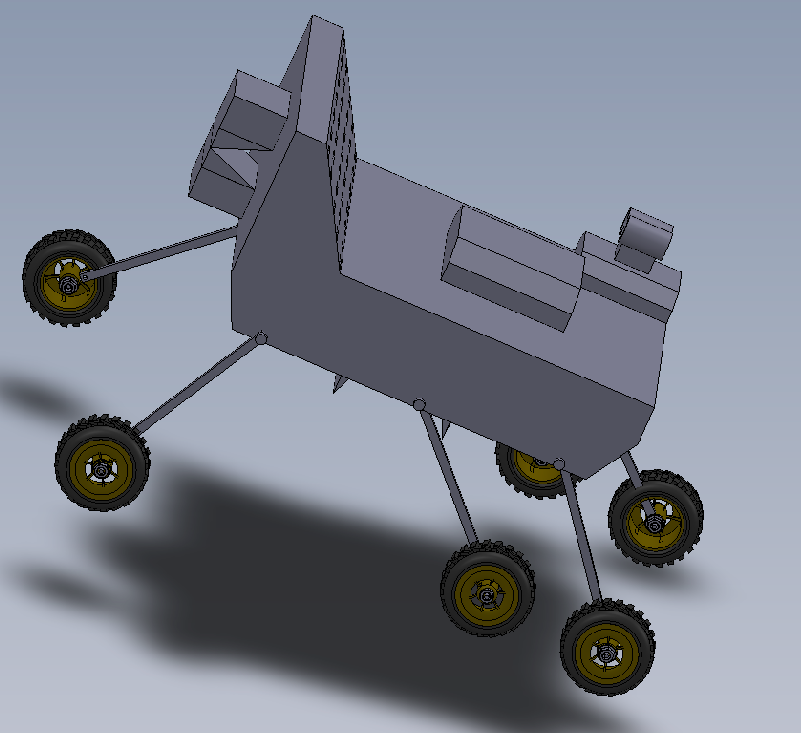
\includegraphics[width=240pt]{Instruments/roverAngle3.png}
   \caption{The 3rd angle of the rover's CAD model}
\end{figure} 

%5.1.2
\subsubsection{ Describe the payload subsystems (if applicable) that are required to
accomplish the payload objectives}
\textbf{Visual System: }The visual system for the probe will consist of a combination of Arduino and Raspberry Pi components. The reason for choosing this route is due to the customizable nature, light weight, low power requirements, and easy attainability of these instruments. A list of parts chosen and their basic function is outlined in figure 30. 
\begin{figure*}
  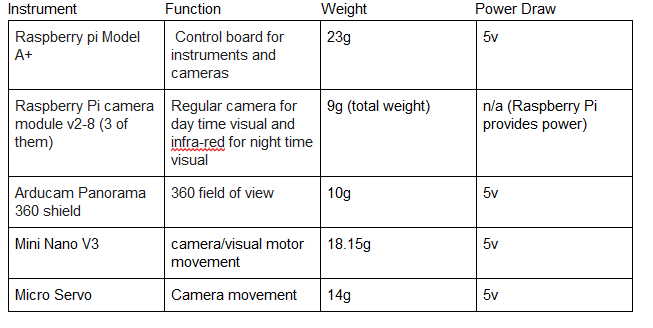
\includegraphics[width=\textwidth]{Instruments/5_1_2_visualSystem.png}
   \caption{The components of the visual system}
\end{figure*} 
There are several pros and cons in choosing such a system. Some of the pros have already been stated. The system is lightweight with the total being less than \begin{math} \frac{1}{4} \end{math} kg. The power draw is low enough to be run on solar panels during the day and lithium batteries during the night. The duality of the camera, with both a normal and infrared lens, leads to visibility for both day and night. The equipment is both cost friendly and easily accessible. 
The main con is the fragility of the system. There is a physical fragility as well as a system fragility. If either the arduino, ribbon cable, raspberry pi cease to function, the entire visual system fails. If one of the cameras fail, an entire field of vision is lost. The small size of each of the components is both a benefit for size and weight requirements, and a drawback as it decreases the overall durability. 

\textbf{"Dust Brush": }This device will be attached to the arm of the APXS. A simple, lightweight motor will turn two drills that have a material not unlike broom bristles on them. As the motor spins the drills, the bristles push dust off the surface, much like a motorized broom. This prevents the samples the APXS takes from being obscured by the Martian dust that is prevalent throughout the surface. 

%5.1.3
\subsubsection{Describe the performance characteristics for the system (and subsystems
if applicable) and determine the evaluation and verification metrics}
Each of the systems have a pass or fail status, since the specifications of the mission don’t allow for much in the terms of backups in case of any failures.  If the APXS is damaged beyond function, the mission is a failure. If the MGPR is snapped or broken, the mission is a failure. While the mission can go on if a subsystem fails, it will certainly not be as efficient and the data not as accurate. Everything will need to go according to plan the first time.

Each of the components of the subsystems need to be tested and make sure that they can function with a safety factor to give a little wiggle room in case something is slightly off.  For example, if the calibration of the APXS gets changed during the landing process, a program needs to be able to attempt to fix it.  Creating a rubric for exactly what each system and subsystem needs to do is important.  If any piece of equipment can not accomplish that, then the design needs to be reworked until the subsystem can accomplish the mission.

\begin{figure*}
  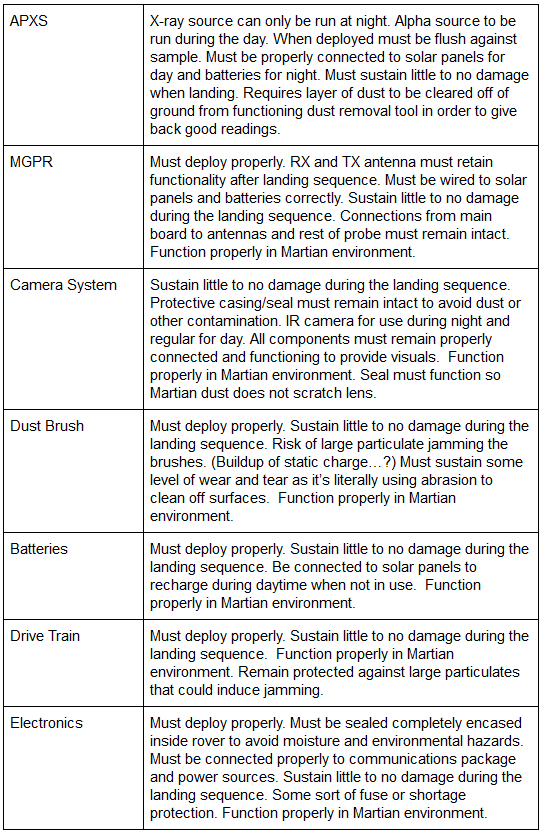
\includegraphics[width=400pt]{Instruments/PayloadPerformanceCharacteristics.png}
   \caption{Payload performance characteristics}
\end{figure*} 

%5.1.4
\subsubsection{Describe the verification plan and its status}
Upon clearing all testing procedures we can certify that all the systems and subsystems can meet and exceed all the hazards and challenges that the payload will meet.  We have set a bar of a safety factor of 30\%. This means that the payload is designed to exceed the requirements of operating safely on Mars by 30\%. By creating the subsystems to exceed the minimum requirements we can safely say that if the subsystems do not outright fail that they will be able to do their job.

%5.1.5
\subsubsection{Describe preliminary integration plan}
The preliminary integration plan with the EDL system, is to have the payload sit inside of it. It would be fastened to the 'walls,' of the EDL system, with motorized latches that would let the payload loose upon deployment. 

%5.1.6
\subsubsection{ Determine the precision of instrumentation and repeat-ability of the
measurements}
The APXS, while highly accurate, is not without its drawbacks. Large concentrations of the element have a low error rate, but the closer the concentration is to the APXS detection limit there is a higher liklihood of errors, up to 50\%\cite{bruckner2003refined}. However, hte more readings of an area, the better understanding of the character of the surrounding elements and the margin of error is minimized. Decreasing the margin of error is an open research area and many suggestions are likely to be available to attempt as well. 

The ground penetrating radar has a fairly moderate resolution of 1.5m.  At shorter distances of up to 5m, the GPR has an increased resolution of 15cm. This increased resolution can provide valuable information about the ice to regolith ratio and the future accessibility of ice for feedstock in crewed Mars missions. MGPR can also give further information about landforms in the Moreux Crater that illustrate the history of glacial movement. 

The measurements this mission is taking is repeatable ad infinitum. As long as all the equipment continues to function properly, the rover can continue to take readings. While the longer the mission operates, the less valuable the data becomes, the team believes it is good mission design that the machine can take readings until the necessary data is collected. 

%5.2
\subsection{Payload Concept Features and Definition}

%5.2.1
\subsubsection{Creativity and originality}
This team feels like this mission is suitably creative and original. While legacy instruments and descent methods were used, the exact combination present has not been used before. One example of this that illustrates the creativity present in the design is the EDL system. The EDL system is a pyramid shape that encapsulates the payload. The pyramidal shape allows the two sections of the payload to be nearly completely modular. In addition, the shape gives another huge benefit: the fact that the probe can land in any configuration and the EDL system will still ensure that it still deploys correctly regardless of orientation. 

%5.2.2
\subsubsection{Uniqueness or significance}
Several quantifiers are evidence of the uniqueness and significance of this mission design. The team composition is one factor. The entire team is comprised entirely of undergraduates from a variety of fields and expertise. The specifications given for the mission document also gave way to its uniqueness. While general guidance was given on how to approach the mission design, overall the team was given only a few specifications. A question was presented and Team 25 has done it's best to answer that question within the provided restrictions.

The significance of the proposed questions on the characterization of ice at Mars is large. A successful execution of this mission would be very significant. It would help confirm or deny the chosen landing site's human colony potential due to the presence (or lack of) ice that could be water feedstock. This is an important step in what could be the largest accomplishment humanity will achieve in this team's lifetime: landing a crewed mission on and beginning colonization of Mars.


%5.2.3
\subsubsection{Suitable level of challenge}
The weight limit on the probe proved to be one of the largest challenges faced. Given the weight limit, time frame, experience level, and broadness of mission specification,Team 25 believes it has adequately met the challenge presented. The payload concept provides sufficient information to either confirm or deny Moreux Crater as a site worth further investigation as a source of water for later crewed Mars missions. Successful completion of this mission would be an important deciding factor in the first crewed mission to Mars. 

%Basically, does this payload concept provide the best, optimized science return for the money? You are trying to add to the knowledge for preparing Humans to go to Mars! Is your experiment suitable to the level of this challenge in terms of your concept features?

%Begin section VI
\section{\label{sec:level6}Activity Plan}

%6.1
\subsection{Show Status of Activities and Schedule}

%6.1.1
\subsubsection{Budget Plan Cost all items (even free items should be listed with
estimated cost if purchased)}
The budget for this mission is not to exceed \$20 Million. See Appendix A for a budget summary. The budget in it's entirety can be found at \url{ https://docs.google.com/spreadsheets/d/1RBhyTIyYNd3G59kN6SoGBwT-fkixCF3z1GY1jF170vU/edit?usp=sharing}

%6.1.2
\subsubsection{Schedule – L’SPACE Academy 1: This schedule will include all activities from beginning of project to PDR.}
For this mission's planning and organization, a Gantt chart was used. See Appendix B for an example. As the chart is a living document and much too large to show in this report, it will also be linked here and available until at least July of 2019: \url{https://studentswosu-my.sharepoint.com/:x:/g/personal/millerjl2_student_swosu_edu/EfXKIkqJrUFKo3mt6Cu8ExsBv2l2GTwuVSw_EmKcjbSBXQ?e=QZA6bB}

%6.1.3
\subsubsection{Mission Education and Public Outreach Summary}
The diversity of universities represented within the team allow for a relatively far-reaching outreach possibility. For now, the team has planned to speak on their respective campuses about the LSPACE academy and this PDR development. 

%Begin Section VII
\section{\label{sec:level7}Conclusion}

%7.1
\subsection{Summary of Mission}
In conclusion, this mission would fulfill a need. In the near future, NASA and other space agencies plan on going to Mars, and sending humans there for extended periods. To do this, those people will need water to survive, and the most efficient way to obtain water is a feed stock on site. This mission will enable future mission planners to have a much better idea at what kind of feed stock possibilities already exist at the planned location. The fact that this mission is low cost means it could be repeated several times at other locations as well. 

To summarize this mission, the lander would exit a mars orbiter on a trajectory to the landing site. Once it enters the atmosphere, the heat shield absorbs the friction heat and is detached when used up. The parachutes deploy, and are detached at a pre-determined altitude. The airbags inflate, allowing for a ballistic landing. Once these airbags deflate, the lander can deploy, righting itself if it needs to. Then the experiment can begin. The mini ground penetrating radar will be able to determine the composition of the crust beneath it, up to 50M. This will give a good idea of the quantity and depth of most of the ice. The APXS will give a good idea to the chemical makeup and potability of the water on-site. The mission duration can last at least three nights before battery power is no longer guaranteed, but the solar panels give an indefinite mission life. That gives an ample amount of time to collect data. 

%7.1.1
\subsubsection{Progress on mission formulation and design up to CDR}
Of course, nothing is perfect, and this preliminary design review is no exception. This document would by no means be stagnant, and would continue evolving into phase B, and the formulation of the CDR. There are a few things the team would like to revise. 

The biggest issue the team ran into is that the team was severely lacking in a chemistry expert, a niche that would have benefited the mission formulation immensely. It would be to the benefit of this PDR to have such an expert review this document, and collaborate on how better to collect data and structure the mission. Especially regarding APXS instrument, such help would be extremely useful.

From here, the next step would be verifying this document with peers and experts, and modifying it. This process would continue until the deadline of this mission's submission arrived.

%7.1.2
\subsubsection{Testing Results and mission success outlook}
Does not Apply

\begin{acknowledgments}
We wish to thank the Lucy mission and especially the L'SPACE team for offering this academy and all the encouragement and support they offered along the way. 

We wish to acknowledge the creators of REV\TeX{}, whose \LaTeX{} template helped tremendously in the formation of this document. 
\end{acknowledgments}

\nocite{*}
\bibliography{lspaceteam25}

\appendix

\clearpage
\section{Budget Summary}
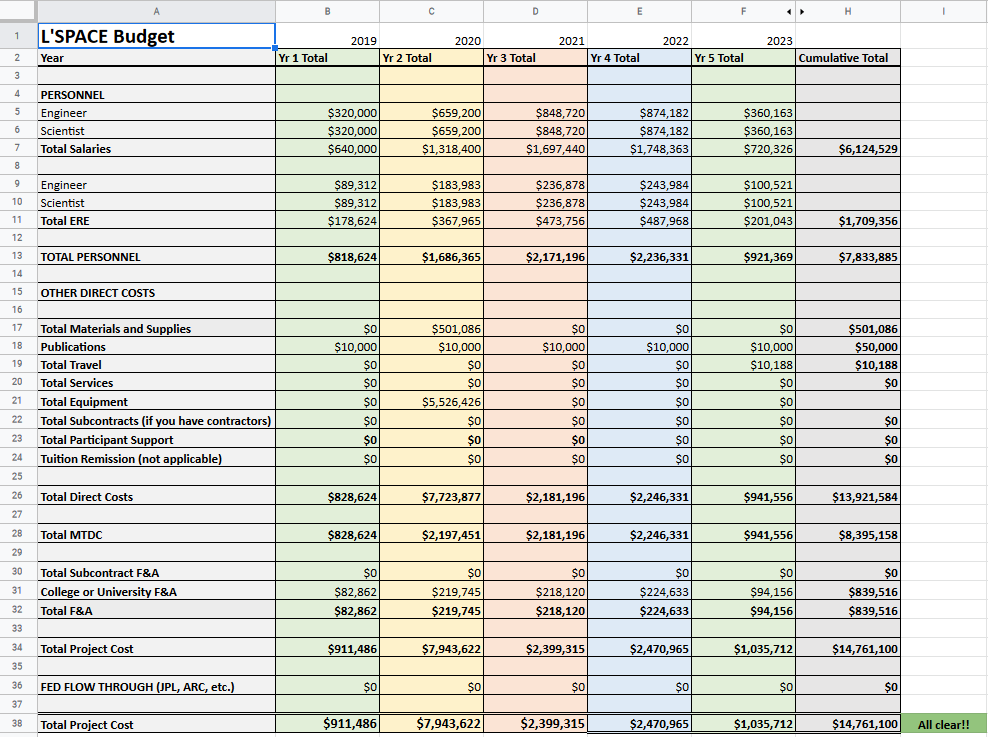
\includepdf{Appendices/Budget.png}
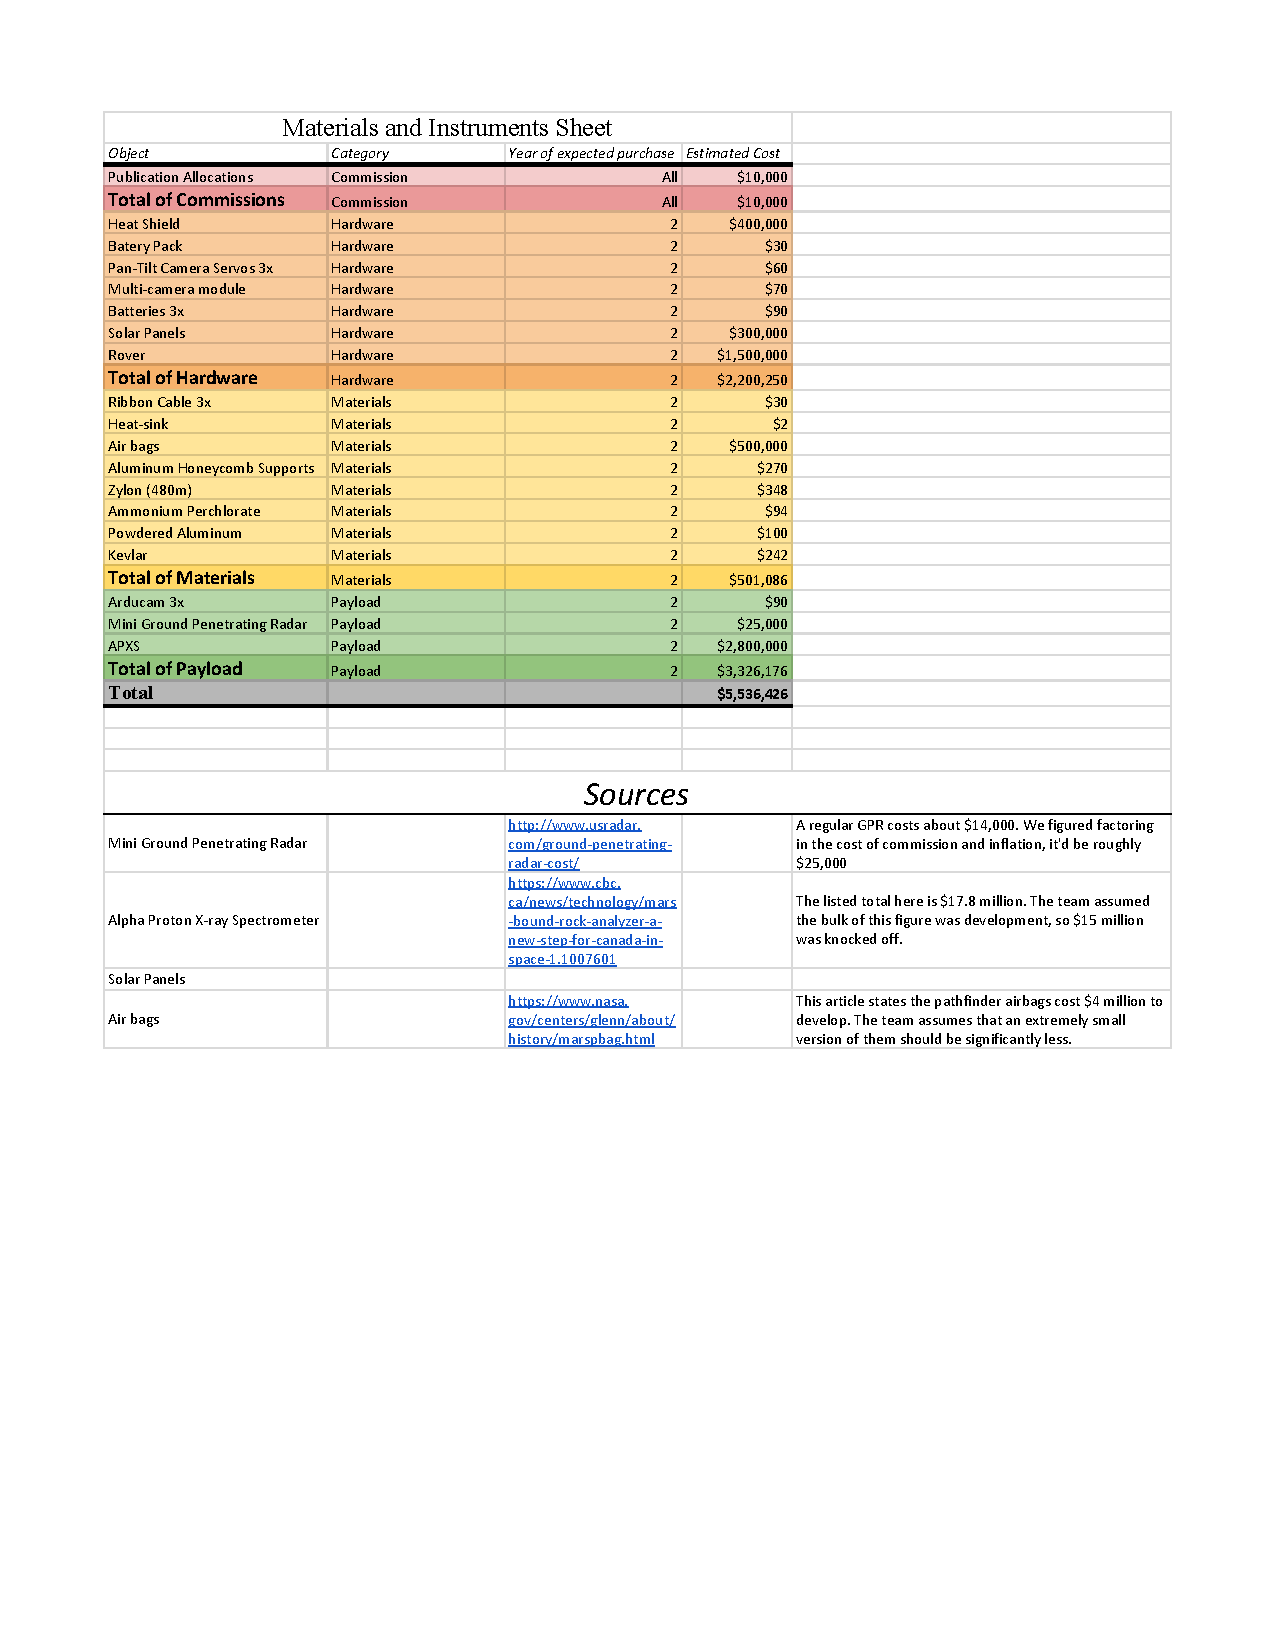
\includepdf{Appendices/L_SPACE_Hardware.pdf}
\clearpage

\section{Project Schedule}
\begin{figure}[h!]
  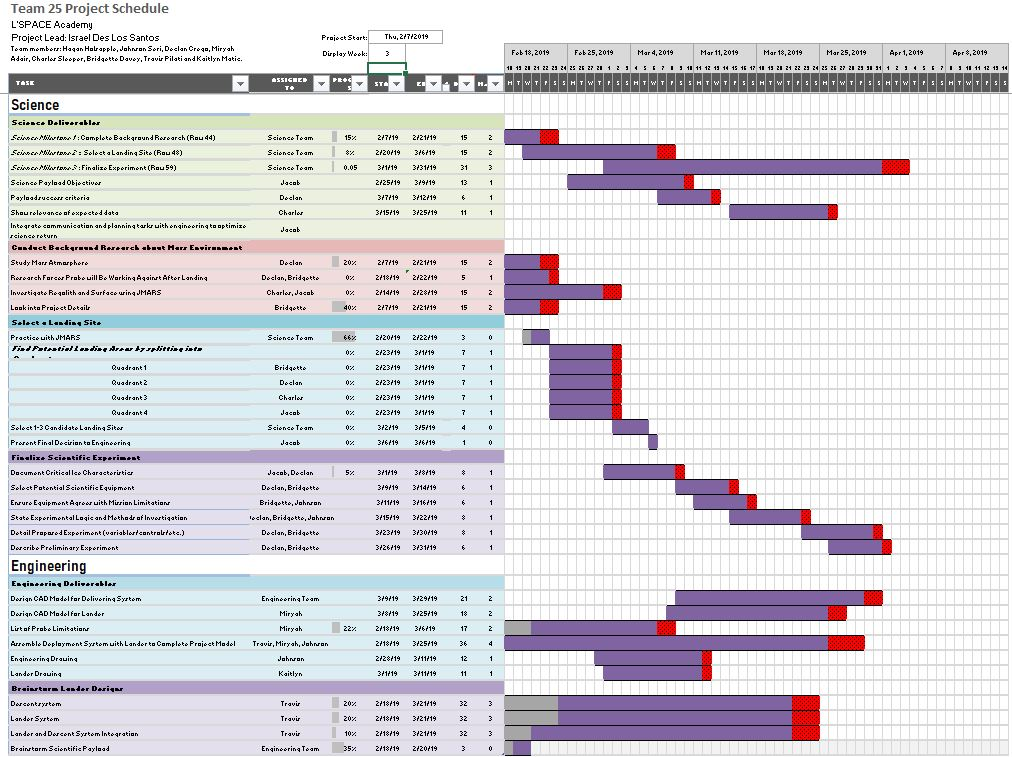
\includegraphics[scale=.85, angle=90]{Appendices/FinishedChart.jpg}
\end{figure} 

\clearpage
p
\section{MSDS}

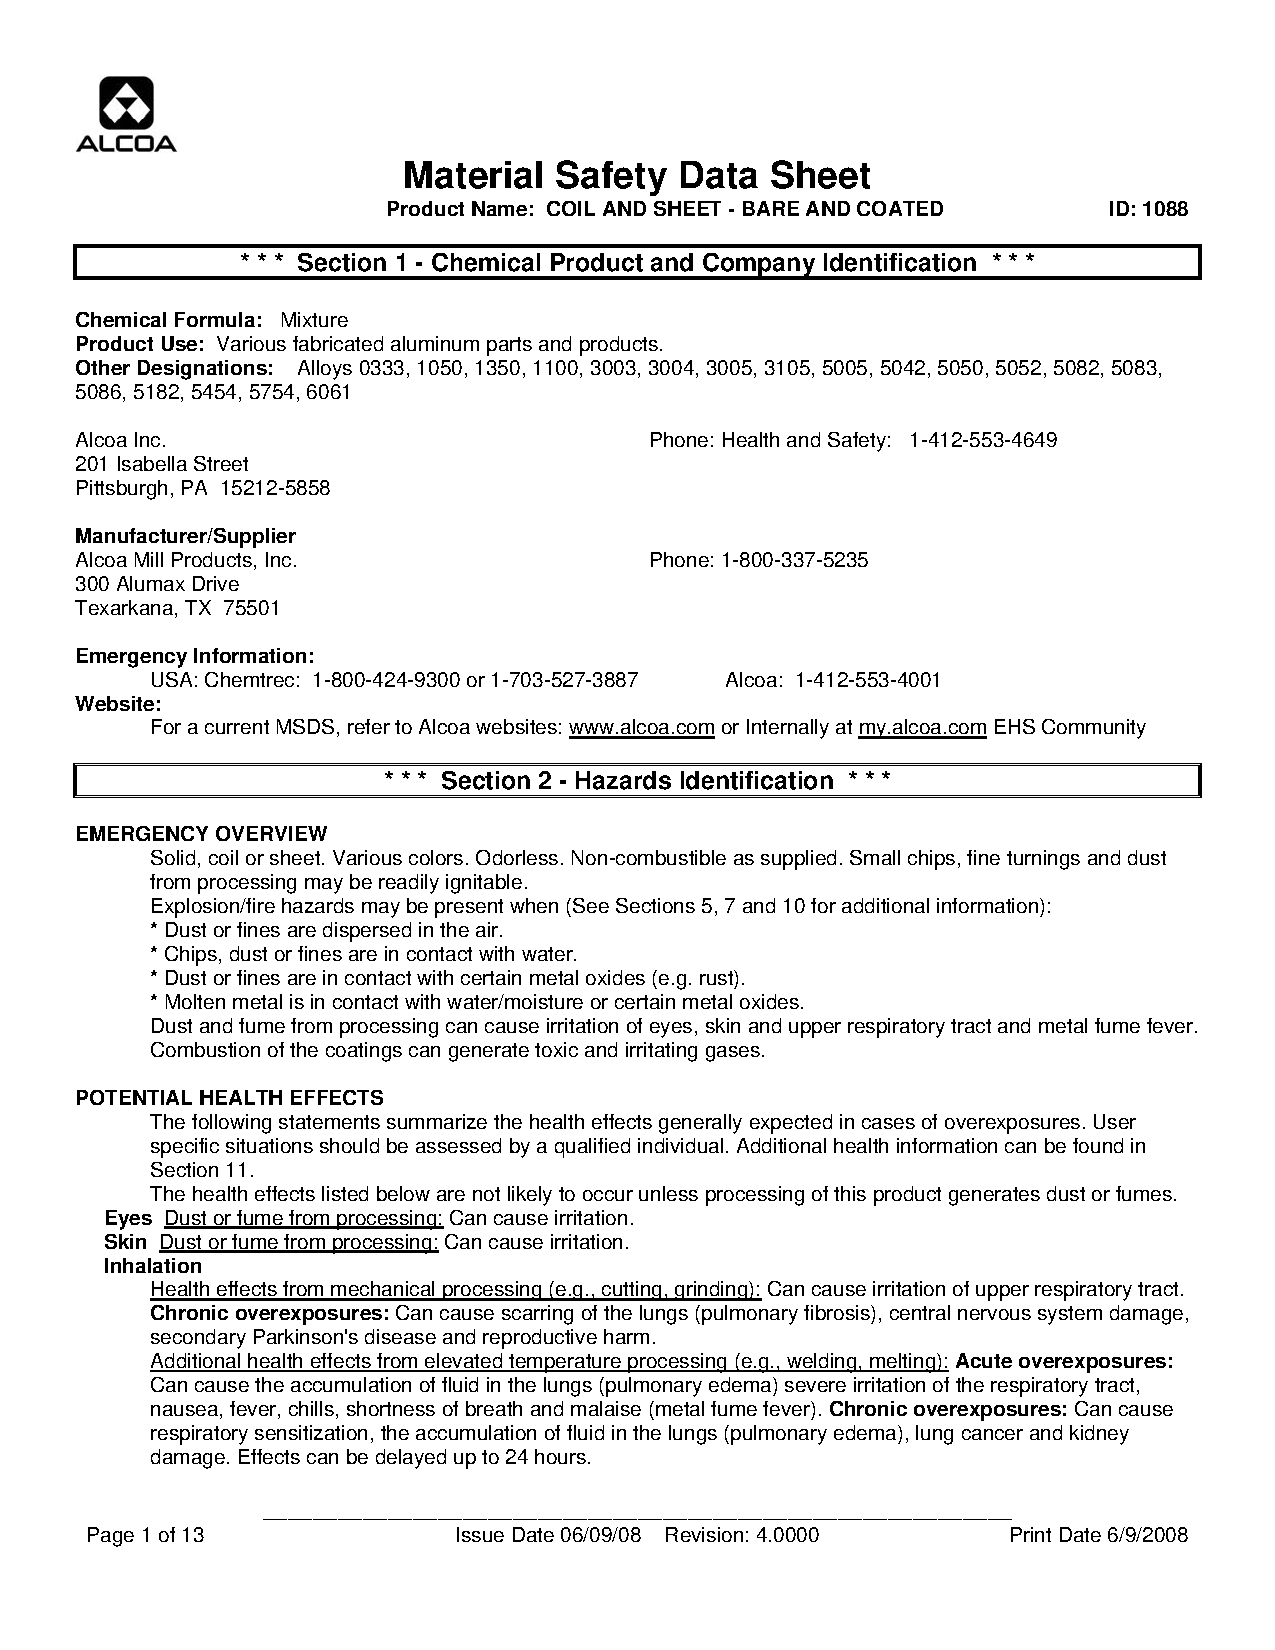
\includepdf[pages=1]{Appendices/MSDS/MSDS-Aluminum.pdf}
\includepdf[pages=2]{Appendices/MSDS/MSDS-Aluminum.pdf}
\clearpage
\includepdf[pages=3]{Appendices/MSDS/MSDS-Aluminum.pdf}
\clearpage
\includepdf[pages=4]{Appendices/MSDS/MSDS-Aluminum.pdf}
\clearpage
\includepdf[pages=5]{Appendices/MSDS/MSDS-Aluminum.pdf}
\clearpage
\includepdf[pages=6]{Appendices/MSDS/MSDS-Aluminum.pdf}
\clearpage
\includepdf[pages=7]{Appendices/MSDS/MSDS-Aluminum.pdf}
\clearpage
\includepdf[pages=8]{Appendices/MSDS/MSDS-Aluminum.pdf}
\clearpage
\includepdf[pages=9]{Appendices/MSDS/MSDS-Aluminum.pdf}
\clearpage
\includepdf[pages=10]{Appendices/MSDS/MSDS-Aluminum.pdf}
\clearpage
\includepdf[pages=11]{Appendices/MSDS/MSDS-Aluminum.pdf}
\clearpage
\includepdf[pages=12]{Appendices/MSDS/MSDS-Aluminum.pdf}
\clearpage
\includepdf[pages=13]{Appendices/MSDS/MSDS-Aluminum.pdf}

\clearpage
\includepdf[pages=1]{Appendices/MSDS/Kevlar-MSDS.pdf}
\clearpage
\includepdf[pages=2]{Appendices/MSDS/Kevlar-MSDS.pdf}
\clearpage
\includepdf[pages=3]{Appendices/MSDS/Kevlar-MSDS.pdf}
\clearpage
\includepdf[pages=4]{Appendices/MSDS/Kevlar-MSDS.pdf}
\clearpage
\includepdf[pages=5]{Appendices/MSDS/Kevlar-MSDS.pdf}
\clearpage
\includepdf[pages=6]{Appendices/MSDS/Kevlar-MSDS.pdf}
\clearpage
\includepdf[pages=7]{Appendices/MSDS/Kevlar-MSDS.pdf}

\clearpage
\includepdf[pages=1]{Appendices/MSDS/rdxmsds.pdf}
\clearpage
\includepdf[pages=2]{Appendices/MSDS/rdxmsds.pdf}
\clearpage
\includepdf[pages=3]{Appendices/MSDS/rdxmsds.pdf}
\clearpage
\includepdf[pages=4]{Appendices/MSDS/rdxmsds.pdf}
\clearpage
\includepdf[pages=5]{Appendices/MSDS/rdxmsds.pdf}
\clearpage
\includepdf[pages=6]{Appendices/MSDS/rdxmsds.pdf}

\clearpage
\includepdf[pages=1]{Appendices/MSDS/SodiumazideMSDS.pdf}
\clearpage
\includepdf[pages=2]{Appendices/MSDS/SodiumazideMSDS.pdf}
\clearpage
\includepdf[pages=3]{Appendices/MSDS/SodiumazideMSDS.pdf}
\clearpage
\includepdf[pages=4]{Appendices/MSDS/SodiumazideMSDS.pdf}
\clearpage
\includepdf[pages=5]{Appendices/MSDS/SodiumazideMSDS.pdf}
\clearpage
\includepdf[pages=6]{Appendices/MSDS/SodiumazideMSDS.pdf}
\clearpage
\includepdf[pages=7]{Appendices/MSDS/SodiumazideMSDS.pdf}
\clearpage
\includepdf[pages=8]{Appendices/MSDS/SodiumazideMSDS.pdf}

\clearpage

% Produces the bibliography via BibTeX.

\end{document}
%
% ****** End of file aapmsamp.tex ******